\newpage

\chapter{Results}

Here we present the experimental data obtained from the measurements of quantum turbulence. The tuning fork has been immersed in superfluid $\He$ and forced to oscillate at two, geometrically different (in the sense of different velocity profile along the fork's prongs) modes - \textit{fundamental} $ [6380\unit{Hz}] $ and \textit{overtone} $ [40\,000\unit{Hz}] $.

The first part of this chapter is focused on the measurement of vortex line density $ L $ (total length of vortices in unit volume) using the second sound attenuation technique. We will try to find the conditions for production of quantized vortices and also, quantify their amount.

In the second part we will work only with the tuning fork via the applied voltage amplitudes and its current responses. Using the scaled drag coefficient and oscillatory Reynolds number, we will be able to estimate when the drag force acting on the tuning fork becomes non-linear with velocity. This event is a distinct sign of the flow pattern, changing from simple laminar flow of the normal component and purely potential flow of the superfluid component, to something more complex involving some certain form of classical or/and quantum turbulence.

Overall we worked at seven selected temperatures in the two-fluid regime, when both superfluid and normal component amounts are considerable: $ 1.35\unit{K} $, $ 1.55\unit{K} $, $ 1.65\unit{K} $, $ 1.80\unit{K} $, $ 1.95\unit{K} $, $ 2.05\unit{K} $, $ 2.15\unit{K} $.  {\sffamily\textbf{Figure 3.1}} shows the time trace of the temperature inside the cell. Temperatures below $\approx 1.30\unit{K} $ were not stable, so the lowest fixed value was set to $ 1.35\unit{K} $.  


\begin{figure}[h!]
	\centering
	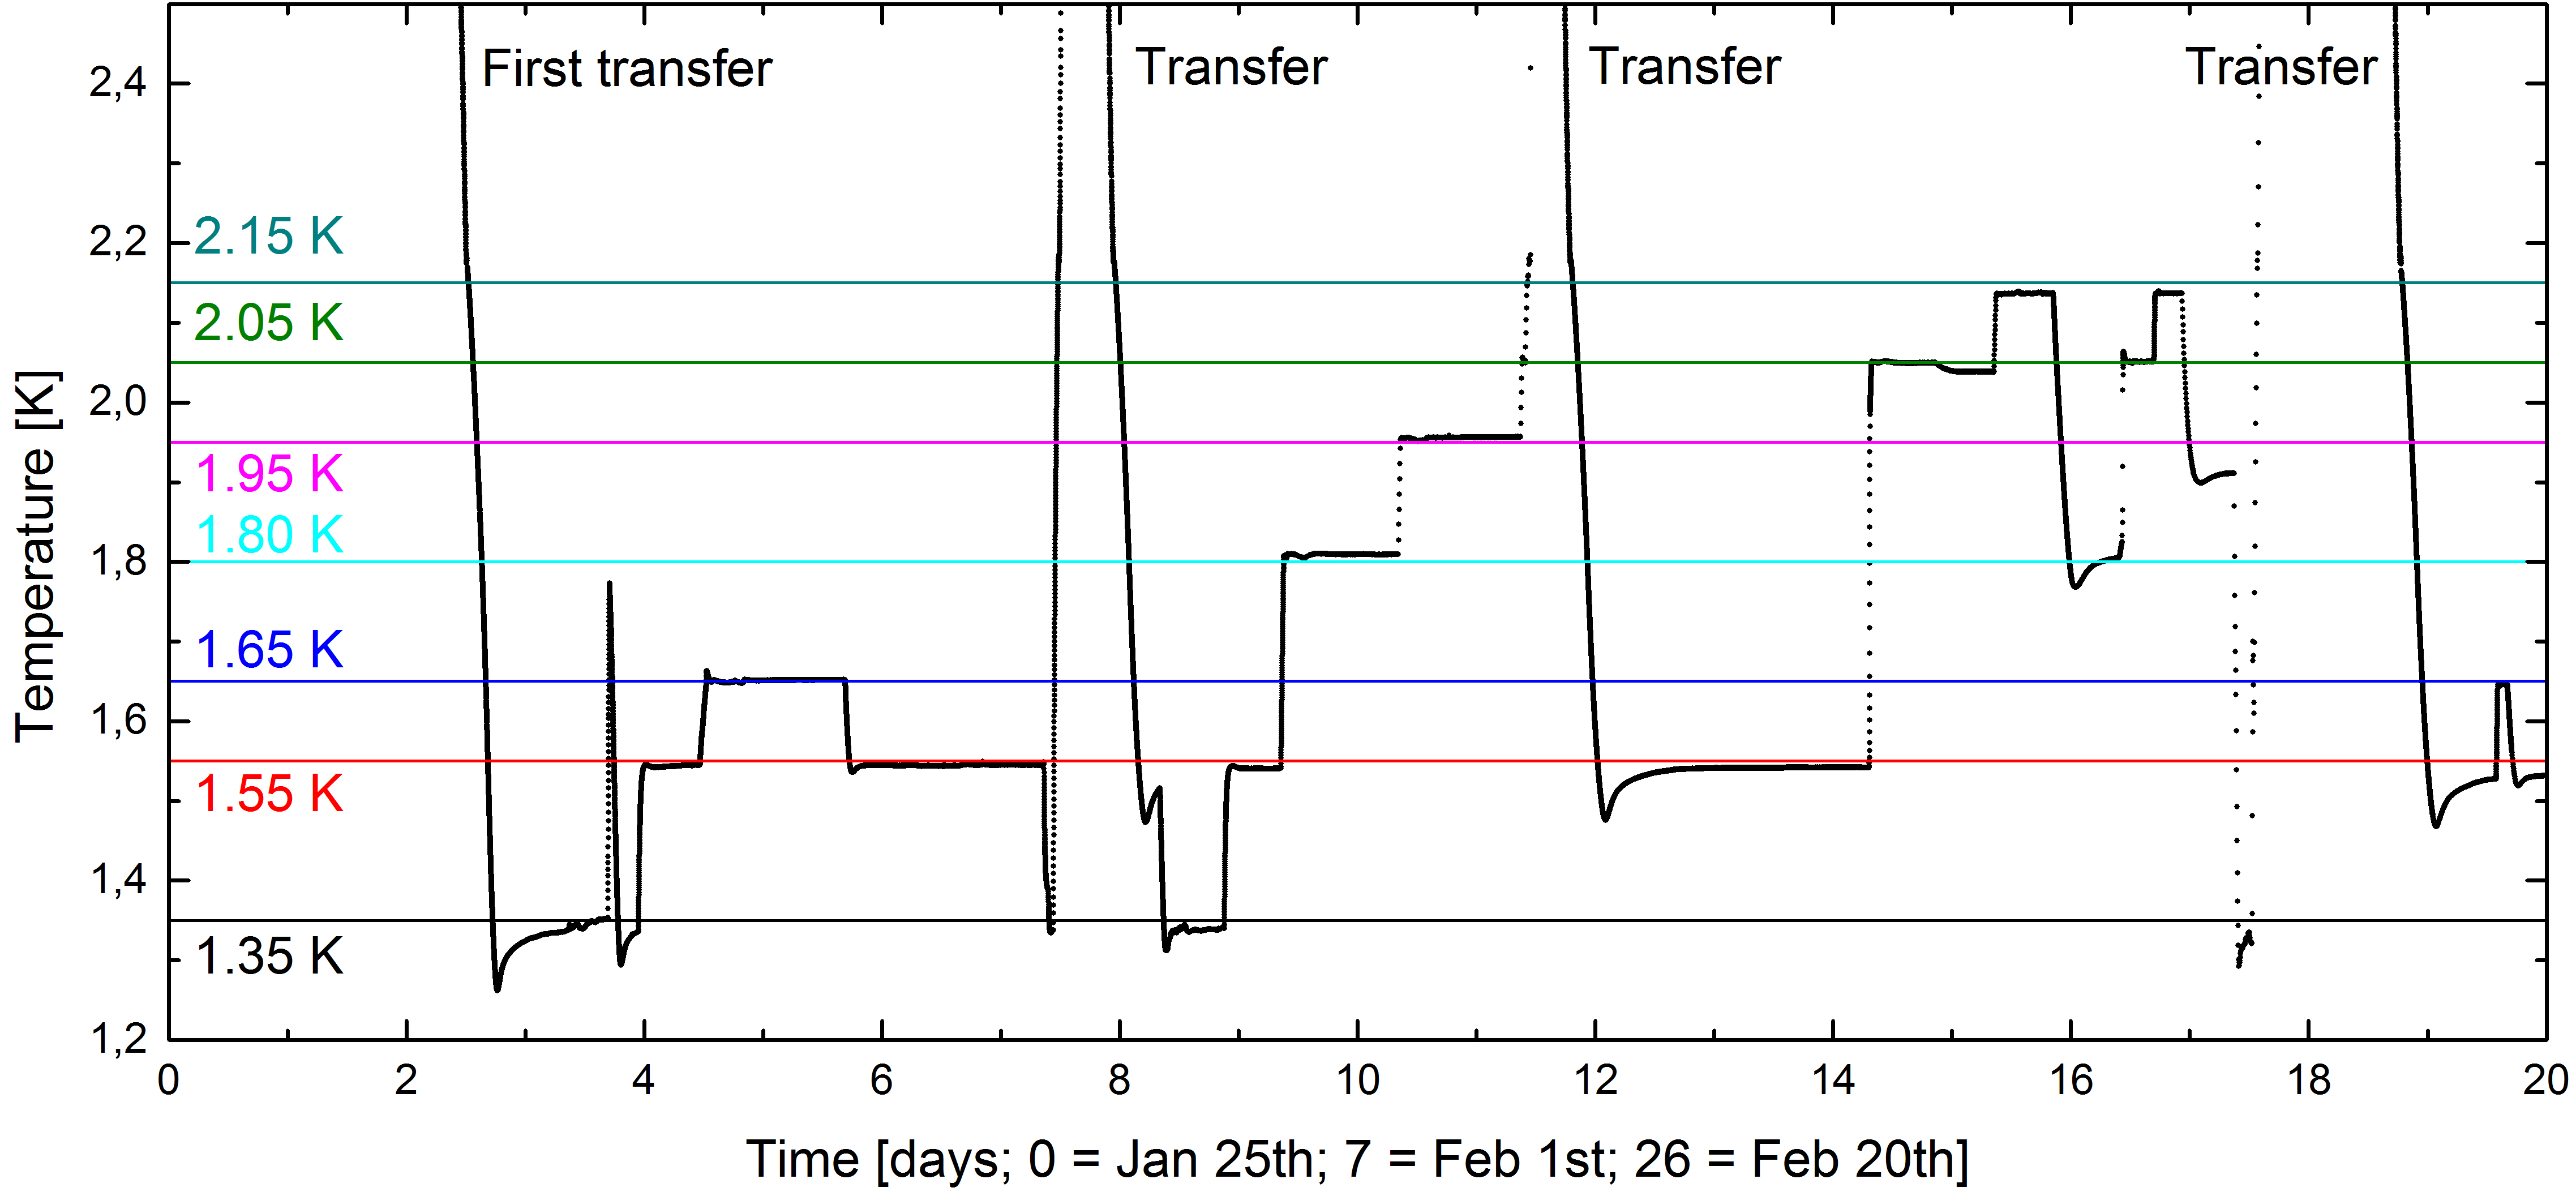
\includegraphics[width=1\textwidth]{graphs/diary}
	\caption{Record of the temperature inside the cryostat. Due to strong evaporation of superfluid helium and relatively long durations of the measurements at each temperature, we had to refill the cryostat three times. Unfortunately, this may have caused some unsystematic behaviour of the tuning fork that manifested after the first refill on Day 8, see the text for details.}
\end{figure}

Due to the prolonged experimental times, we had to refill helium three times, which has likely contributed to unsystematic behaviour of the tuning fork. The fork has yielded different results at the same temperature before and after transfers, especially the refill on Day 8. The data presented in this Thesis should thus be considered as if consisting of two separate categories of measurements: (i) temperatures $ 1.35\unit{K} $, $ 1.55\unit{K} $, $ 1.65\unit{K} $ investigated before Day 8; and (ii) remaining higher temperatures investigated after said transfer. Where we had the choice, we chose to present data measured before the transfer, as we believe that these better reflect the actual properties of the tuning fork and are more useful for comparison (e.g. they compare better with Ref. \cite{lancaster}). Similar effects of different behaviour after the refilling have been observed with other oscillators such as vibrating wires \cite{history}.

We believe that the most likely scenario is that during the transfer and subsequent cooling, some small amount of air entered into the helium bath, solidified, and despite the protection offered by the resonator body, some bits of frozen air found their way towards the surface of the fork and were deposited there. Consequently, the altered tuning fork geometry could have affected the helium flow, especially the exact moment when the drag force becomes non-linear due to a flow instability. While this unfortunate incident means that we are, in principle, working with two different oscillators rather than the exact same tuning fork at all of the investigated temperatures, we believe that the vortex line density measurements correlated with the drag forces acting on the tuning fork still provide very interesting results and are highly valuable not only as a basis for further studies and improvements, but also directly, as a study of oscillatory flows in superfluid helium (regardless of the exact geometry of the vibrating object).


\section{Measurement of Vortex Line Density}

It has already been shown that an object oscillating with sufficient velocity can produce quantized vortices in superfluid helium. For this purpose, we used the tuning fork mounted in the second sound resonator. Our measurement protocol is given in the following steps:

\begin{itemize}
	\item[1)] First, after the desired temperature in the cryostat has been reached, we run the frequency sweep on tuning fork and second sound independently. The tuning fork frequency sweeps are repeated at different drive levels. This gives us the necessary information about the resonance frequencies and widths.
	
	\item[2)] Next we set up the second sound sensors in constant drive mode at its fundamental resonance and allow up to 3 minutes for stabilization.
	
	\item[3)] When this time has passed, we also run the tuning fork in constant drive mode at its resonance (fundamental or overtone) with a given voltage amplitude $ U_0 $ for 3 minutes.
	
	\item[4)] The tuning fork is subsequently turned off and the second sound is again left to stabilize for 2 minutes.

	\item[5)] The values of $ A $ and $ A_0 $ were taken as averages of the periods when the tuning fork was on and off, respectively (see graph in {\sffamily\textbf{Figure 3.2}}).
\end{itemize}


\begin{figure}[h!]
\centering
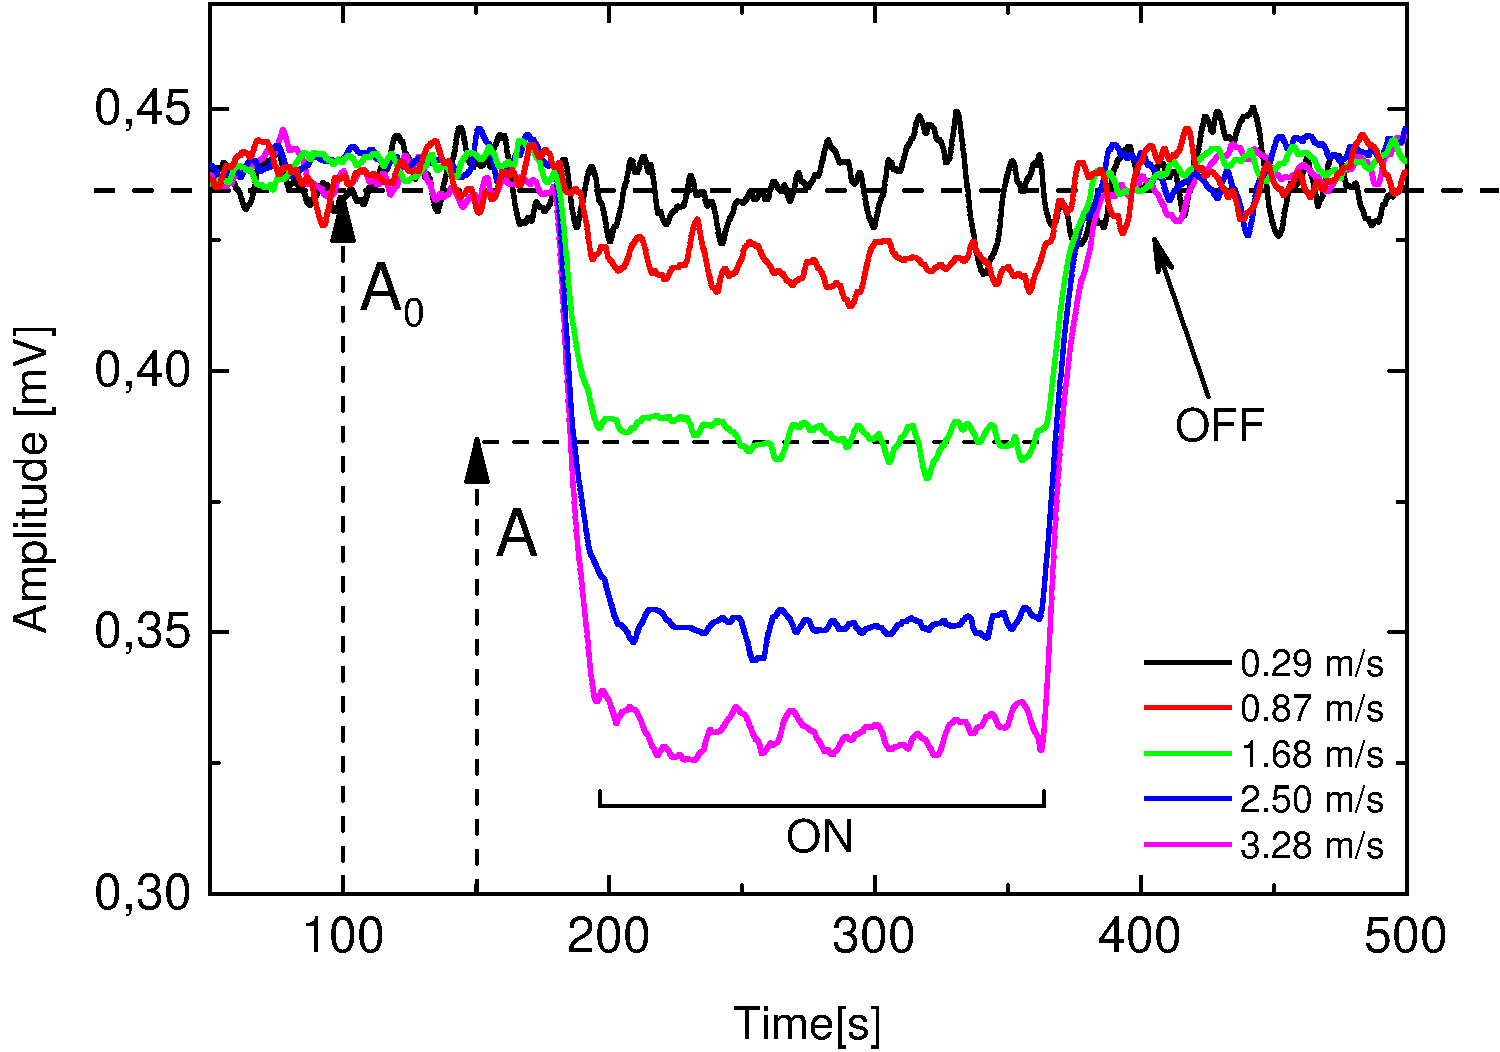
\includegraphics[width=0.75\textwidth]{graphs/Attenuation.pdf}
\caption{An example of second sound attenuation due to the presence of quantized vortices, produced by an oscillating tuning fork at various velocities. "ON" and "OFF" labels describe the state of the tuning fork. The time on the x-axis is measured from the beginning  of each particular run. Values shown in this graph are taken at the temperature $ T=1.95\unit{K} $. The measurement at the velocity of $0.29\unit{m/s}$ corresponds to a vortex line density $L_0 = 3 \times 10^6 \unit{m}^{-2}$ and is taken as an estimate of the sensitivity threshold of our measurement technique.}
\end{figure}

The five aforementioned steps were repeated for several values of voltage applied across the tuning fork, for both fundamental and overtone mode at all six temperatures (all of the above except $ 1.65 \unit{K}$). We have always proceeded from low values of driving voltage to higher ones gradually, so that it is clear, at which point any measurable amount of quantum vortices appears.

By collecting datasets of $ A $, $ A_0 $ and $ \Delta f_0 $ we could estimate the vortex line density $ L $:

\begin{equation}
L = \frac{6\pi \Delta f_0}{B\kappa}\bigg( \frac{A_0}{A} - 1 \bigg)\,,
\label{eq}
\end{equation}

and the fork tip velocity $ v=I/a $, where $ I $ is current response and $ a $ the fork constant. The resulting plot ({\sffamily\textbf{Figure 3.3}}) is shown below.

We should point out that the results for $ L $ as derived in {\sffamily\textbf{Section 1.6}} are valid only for homogeneously and isotropically distributed vortices. The amount of quantized vortices is expected to be higher near the fork than further away from it. Since we utilized the $ 1^{\ind{st}} $ second sound resonant mode, we have, in fact, measured the $ 1^{\ind{st}} $ Fourier component of the vortex line density spatial distribution\cite{Emilfluids}. This is sufficient for the purposes of (roughly) estimating the quantities of quantized vortices produced, but the true values of $ L $ near the tuning fork may differ by some factor and could be obtained only by measurements using several additional second sound resonant modes.

\begin{figure}[h!]
	\centering
	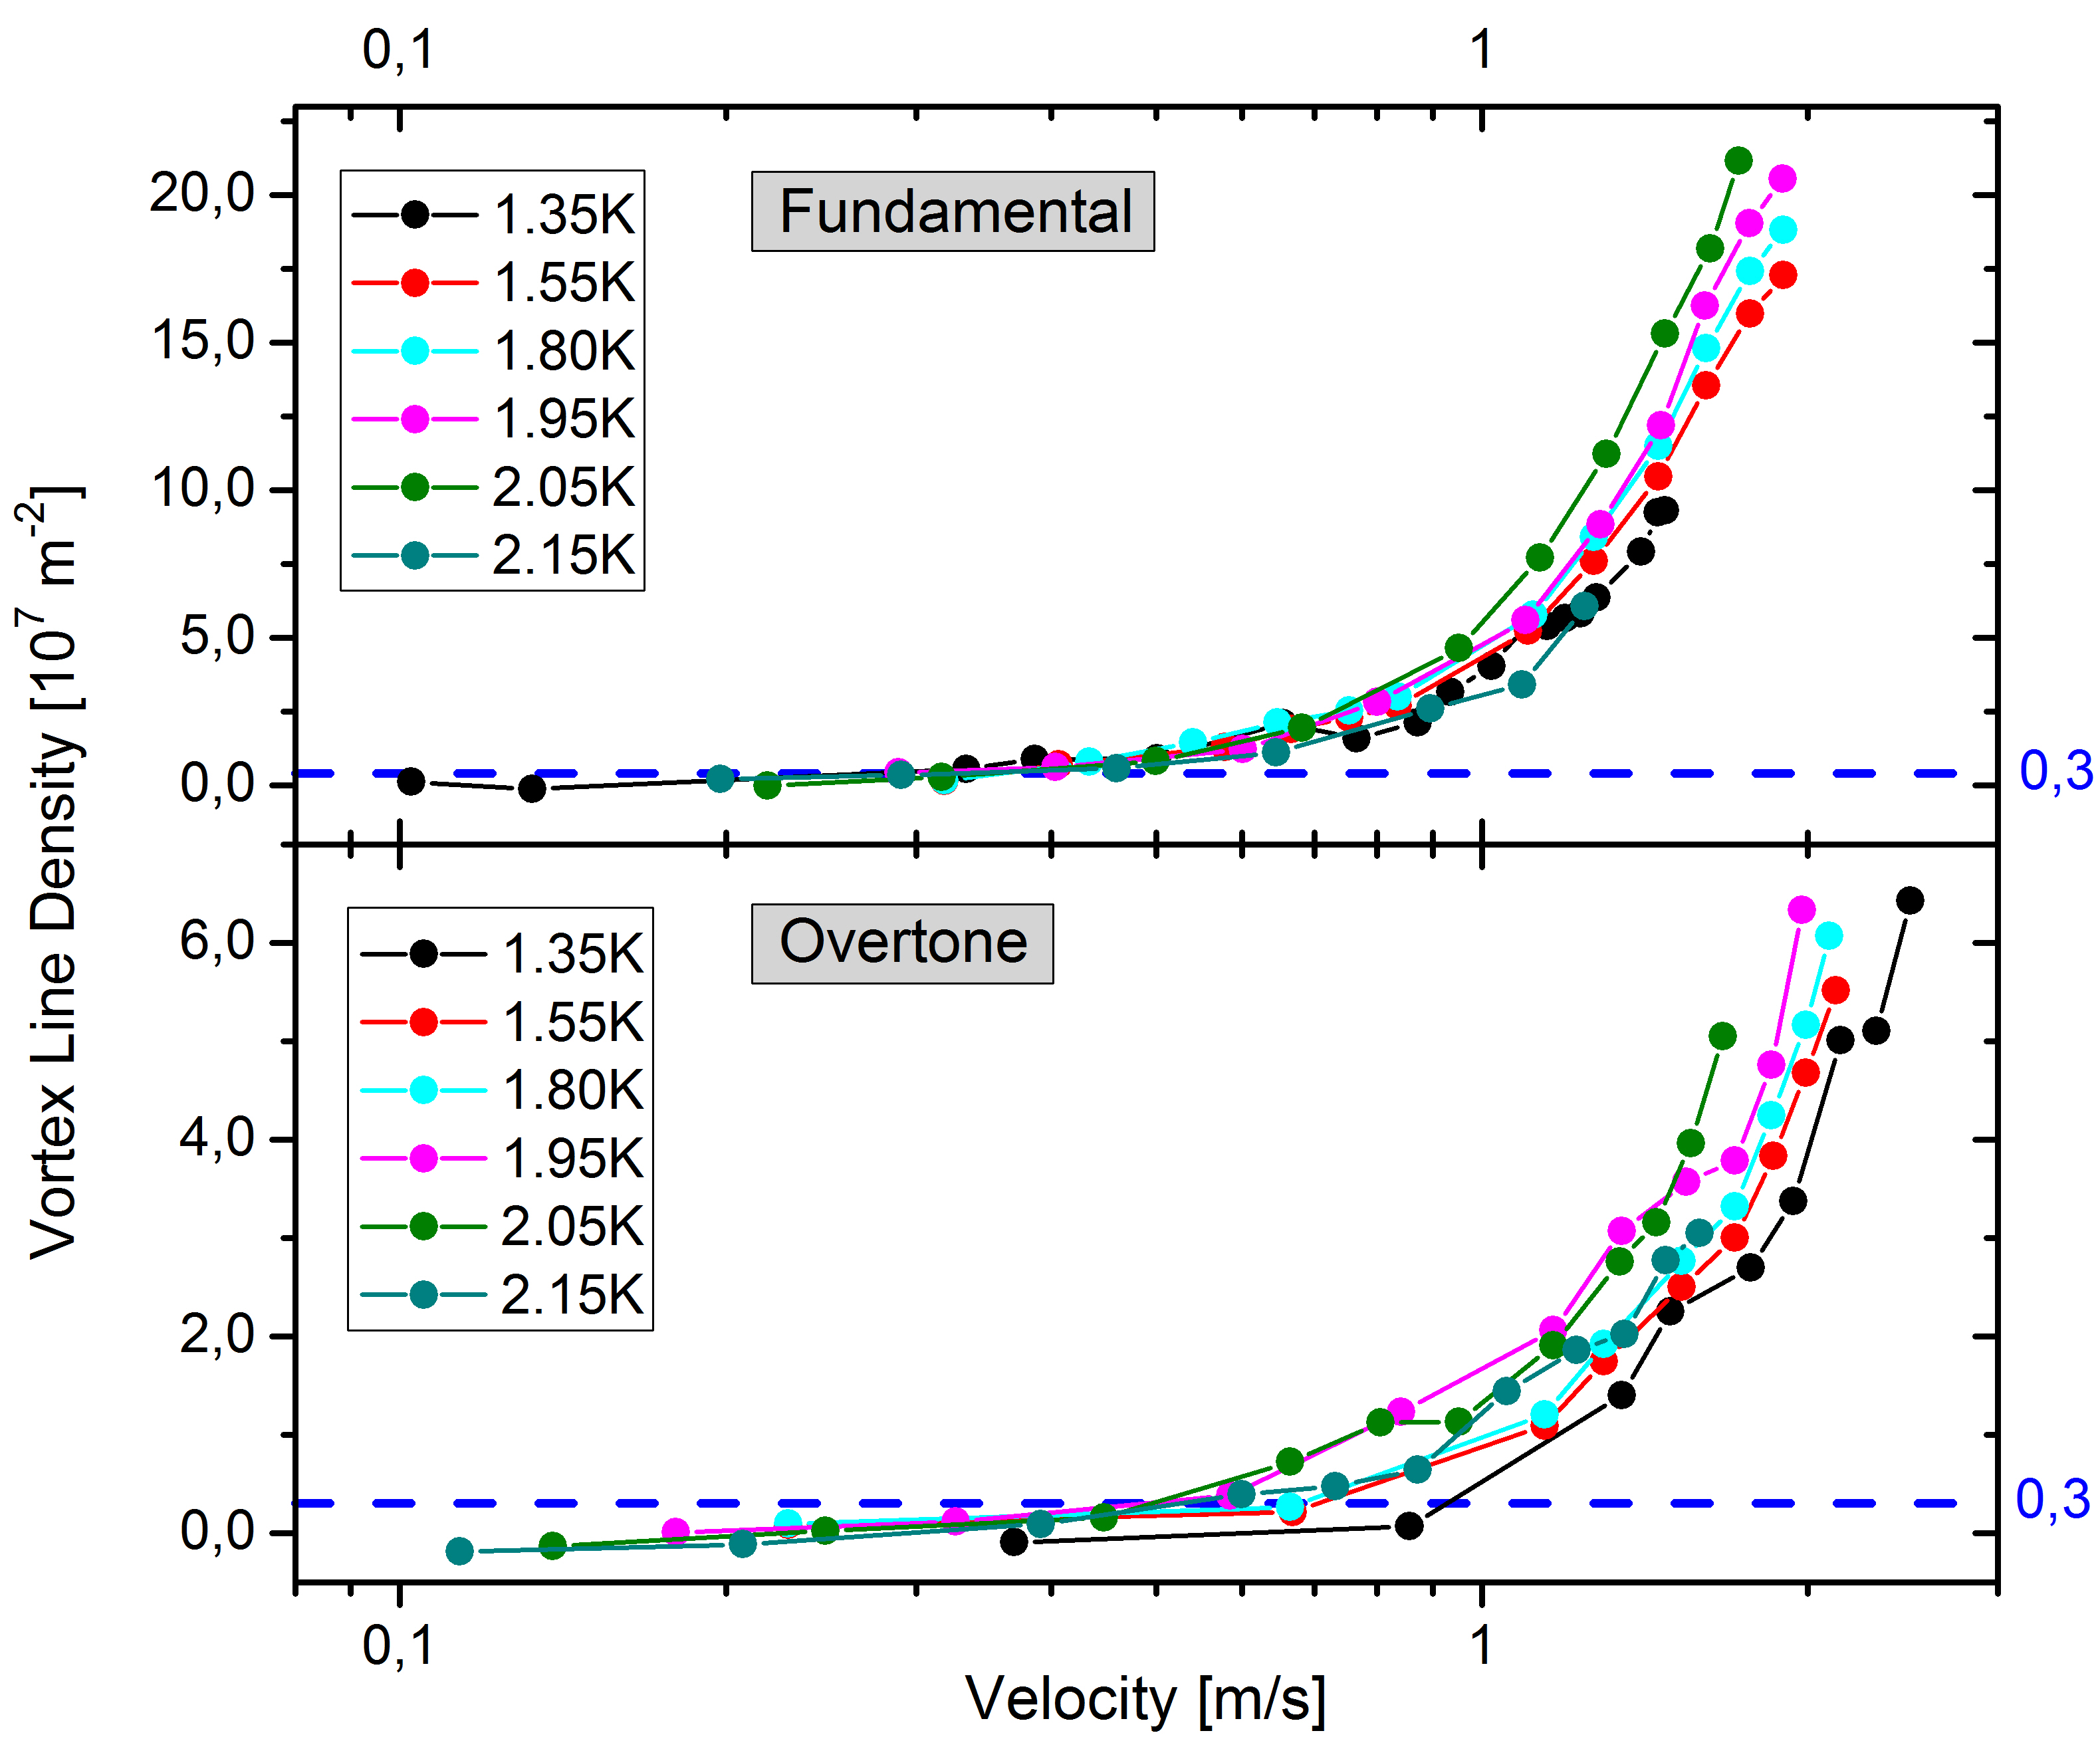
\includegraphics[width=1\textwidth]{graphs/Merged_L_v(abs)}
	\caption{Vortex line density $ L $ against the (logarithmically scaled) peak velocity of the tuning fork $ v $. The \textit{blue dotted line} marks the threshold level $ L_0 \approx 3\cdot 10^6 \unit{m}^{-2} $ introduced in {\sffamily\textbf{Figure 3.2}}, above which the measured vortex line density can be regarded as reliable.}
\end{figure}


Nevertheless, from {\sffamily\textbf{Figure 3.3}} we observe that no significant amounts of vortex lines are produced before a certain critical velocity is exceeded. Furthermore, we find that the amount of quantized vortices produced is temperature-independent and scales only with the velocity of the tuning fork.

After the logarithmic scaling of $ L $ we observe (see {\sffamily\textbf{Figure 3.4}}) that the critical velocities, above which the quantum vortices are produced in much more amounts, are also independent on temperature.
Bearing in mind the sensitivity threshold, we estimate these critical velocities for the fundamental and overtone modes to be $ v_{\ind{c}}^{\ind f} = 0.3 \pm 0.1 \unit{m/s}$, and $ v_{\ind{c}}^{\ind o} = 0.7 \pm 0.2 \unit{m/s} $, respectively. Moreover, as noticed in {\sffamily\textbf{Section 1.10}}, the critical velocity should scale with frequency as $ \propto \sqrt{\kappa\omega} $. From our results we get $ v_{\ind{c}}^{\ind f}/ v_{\ind{c}}^{\ind o} \cdot \sqrt{f_0^{\ind{o}}/f_0^{\ind{f}}} \doteq 1.06 $, which is consistent with the given scaling.

\newpage

\begin{figure}[h!]
	\centering
	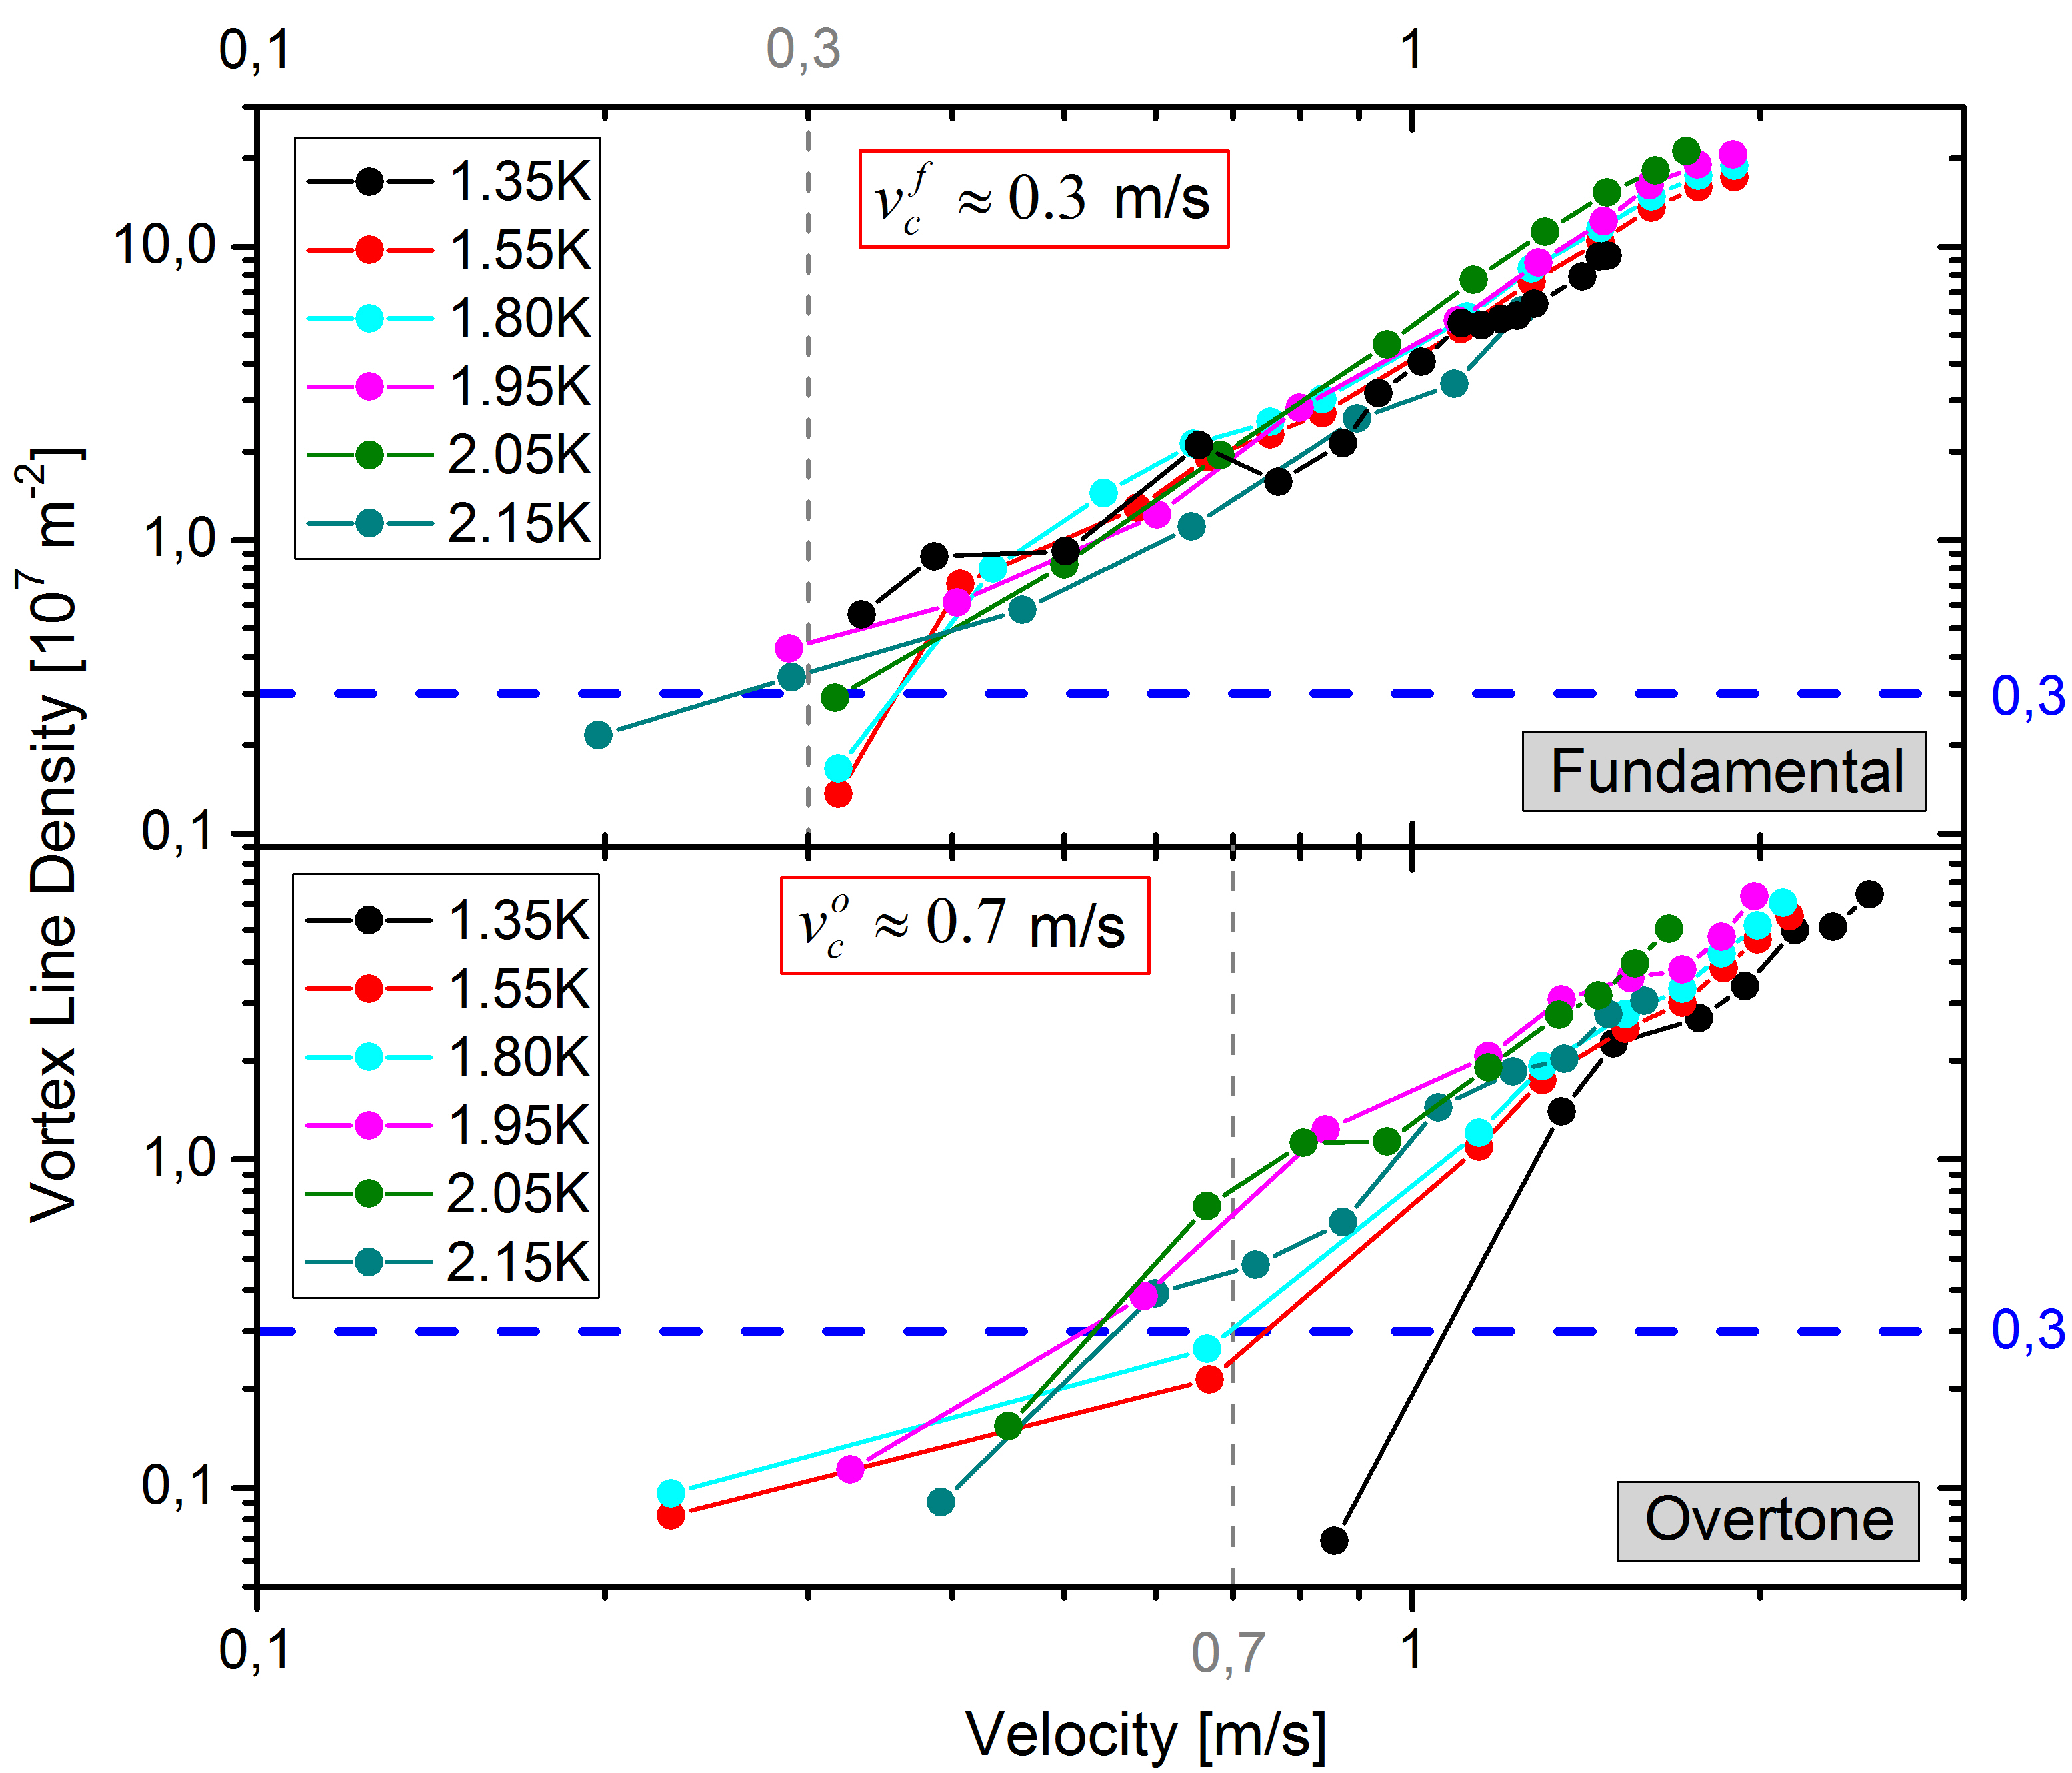
\includegraphics[width=1\textwidth]{graphs/Merged_L_v(log)}
	\caption{Log-log graph of the vortex line density $ L $ against the peak velocity of the tuning fork (the same data as in {\sffamily\textbf{Figure 3.3}}). This graph better illustrates the position of threshold $ L_0 \approx 3\cdot 10^6 \unit{m}^{-2} $ (\textit{blue dashed lines}) and the temperature-independent critical velocities (\textit{grey dashed lines}). The tuning fork peak velocity is determined with an uncertainty of about $ 10\%$ that arises from the electrical calibration procedure\cite{opticalfork}. The vortex line density is affected by a systematic error that is mainly due to the assumption of a homogeneous isotropic tangle in deriving (\ref{eq}) that obviously does not correspond to the vortex tangle produced in the vicinity of the tuning fork.}
\end{figure}


Increasing the sensitivity of the second sound measurement (and thus lowering the threshold level) would allow determining the critical velocities with better accuracy and reduce the scatter in the observed data. Although the design of the second sound resonator and sensors is far from perfect, the current sensitivity is sufficient for a qualitative discussion of the relationship between the obtained vortex line densities and the drag forces acting on the tuning fork.


\newpage

\section{Drag Force Measurements}

All of drag force measurements presented in this Section were done solely with the tuning fork, second sound was not used during the measurement. We have operated the tuning fork in full frequency sweeps, with gradually increasing/decreasing driving voltages. Each of the datapoints in the following graphs is thus obtained from a full frequency sweep of tuning fork around its fundamental or overtone resonance frequency with a given applied voltage $ U_0 $. From such a sweep, the current response $ I $ was measured and for each pair $ \big[U_0,I\big] $ we found the corresponding values of peak applied force and peak velocity $ \big[F,v\big] $ using the calibration formulae from \cite{forks}: $ F = a U_0/2 $, $ v = I/a $.

\begin{figure}[h!]
	\centering
	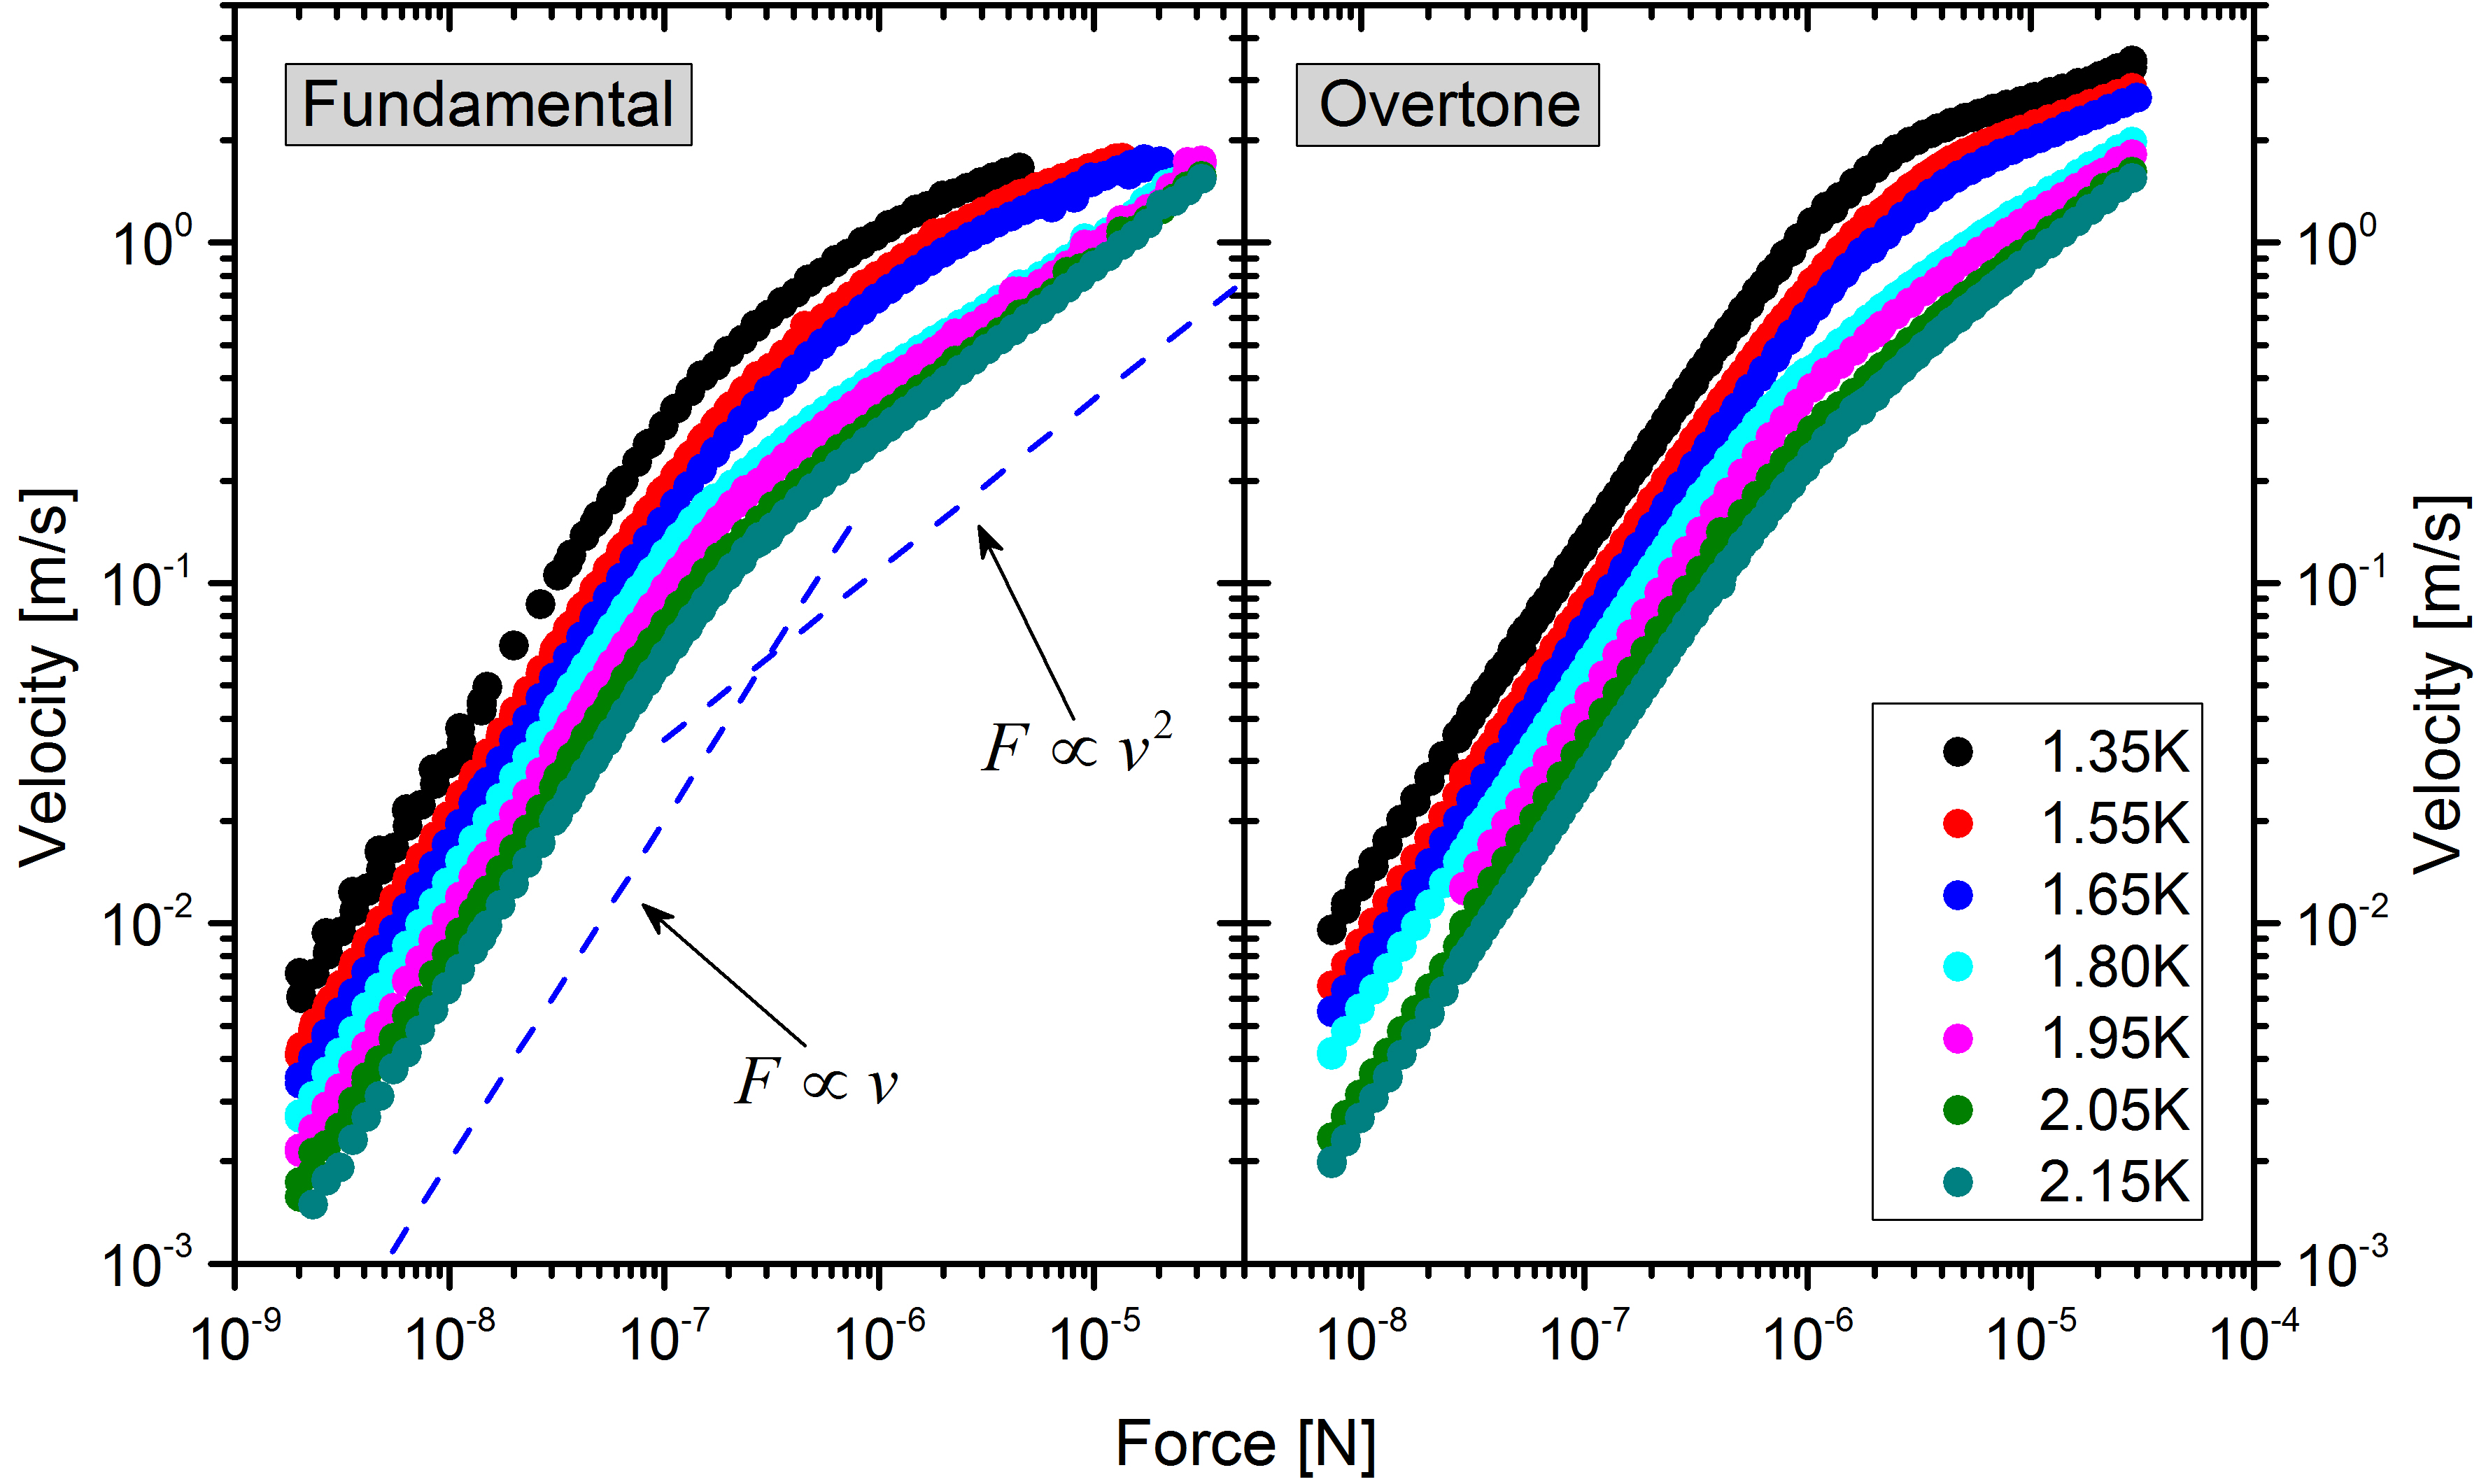
\includegraphics[width=1\textwidth]{graphs/Merged_v_F}
	\caption{Force-Velocity characteristics for the fundamental and overtone modes of our tuning fork at seven different temperatures spanning the two-fluid regime. Apparently, a transition from linear to non-linear drag force occurs at high enough velocities. The \textit{blue dotted lines} sketch the approximate theoretical dependencies for laminar and classical turbulent flow.}
\end{figure}

In {\sffamily\textbf{Figure 3.5}} a transition from linear to non-linear drag is clearly observed. In classical fluid mechanics, the onset of force non-linearity is interpreted as a formation of a wake past the bluff body that encompasses vortical motion of the fluid and may eventually lead to the generation of turbulence. Our case is more complicated since we deal with two (possibly interacting) fluids and hence with two mutually-dependent types of turbulent motion.

It is also apparent that the linear drag force strongly depends on temperature, which reflects the fact that only the normal component contributes to the drag force in laminar flow. At the same time, the superfluid component exhibits purely potential flow, as an ideal fluid might, which results in a zero net contribution to the drag force as per d'Alembert's paradox \cite{landau}. To discuss the scaling properties in greater detail, it is, however, necessary to convert the force and velocity into relevant dimensionless quantities, such as the drag coefficient $ C_{D} = 2F/S\rho v^2 $ and the oscillatory Reynolds number $ \text{Re}_{\delta} = v\rho\delta/\eta $, , where $ S $ stands for the cross-section area of fork perpendicular to the direction of oscillation and $ F $ for the measured drag force.


\begin{figure}[h!]
	\centering
	\vspace{-0.3cm}
	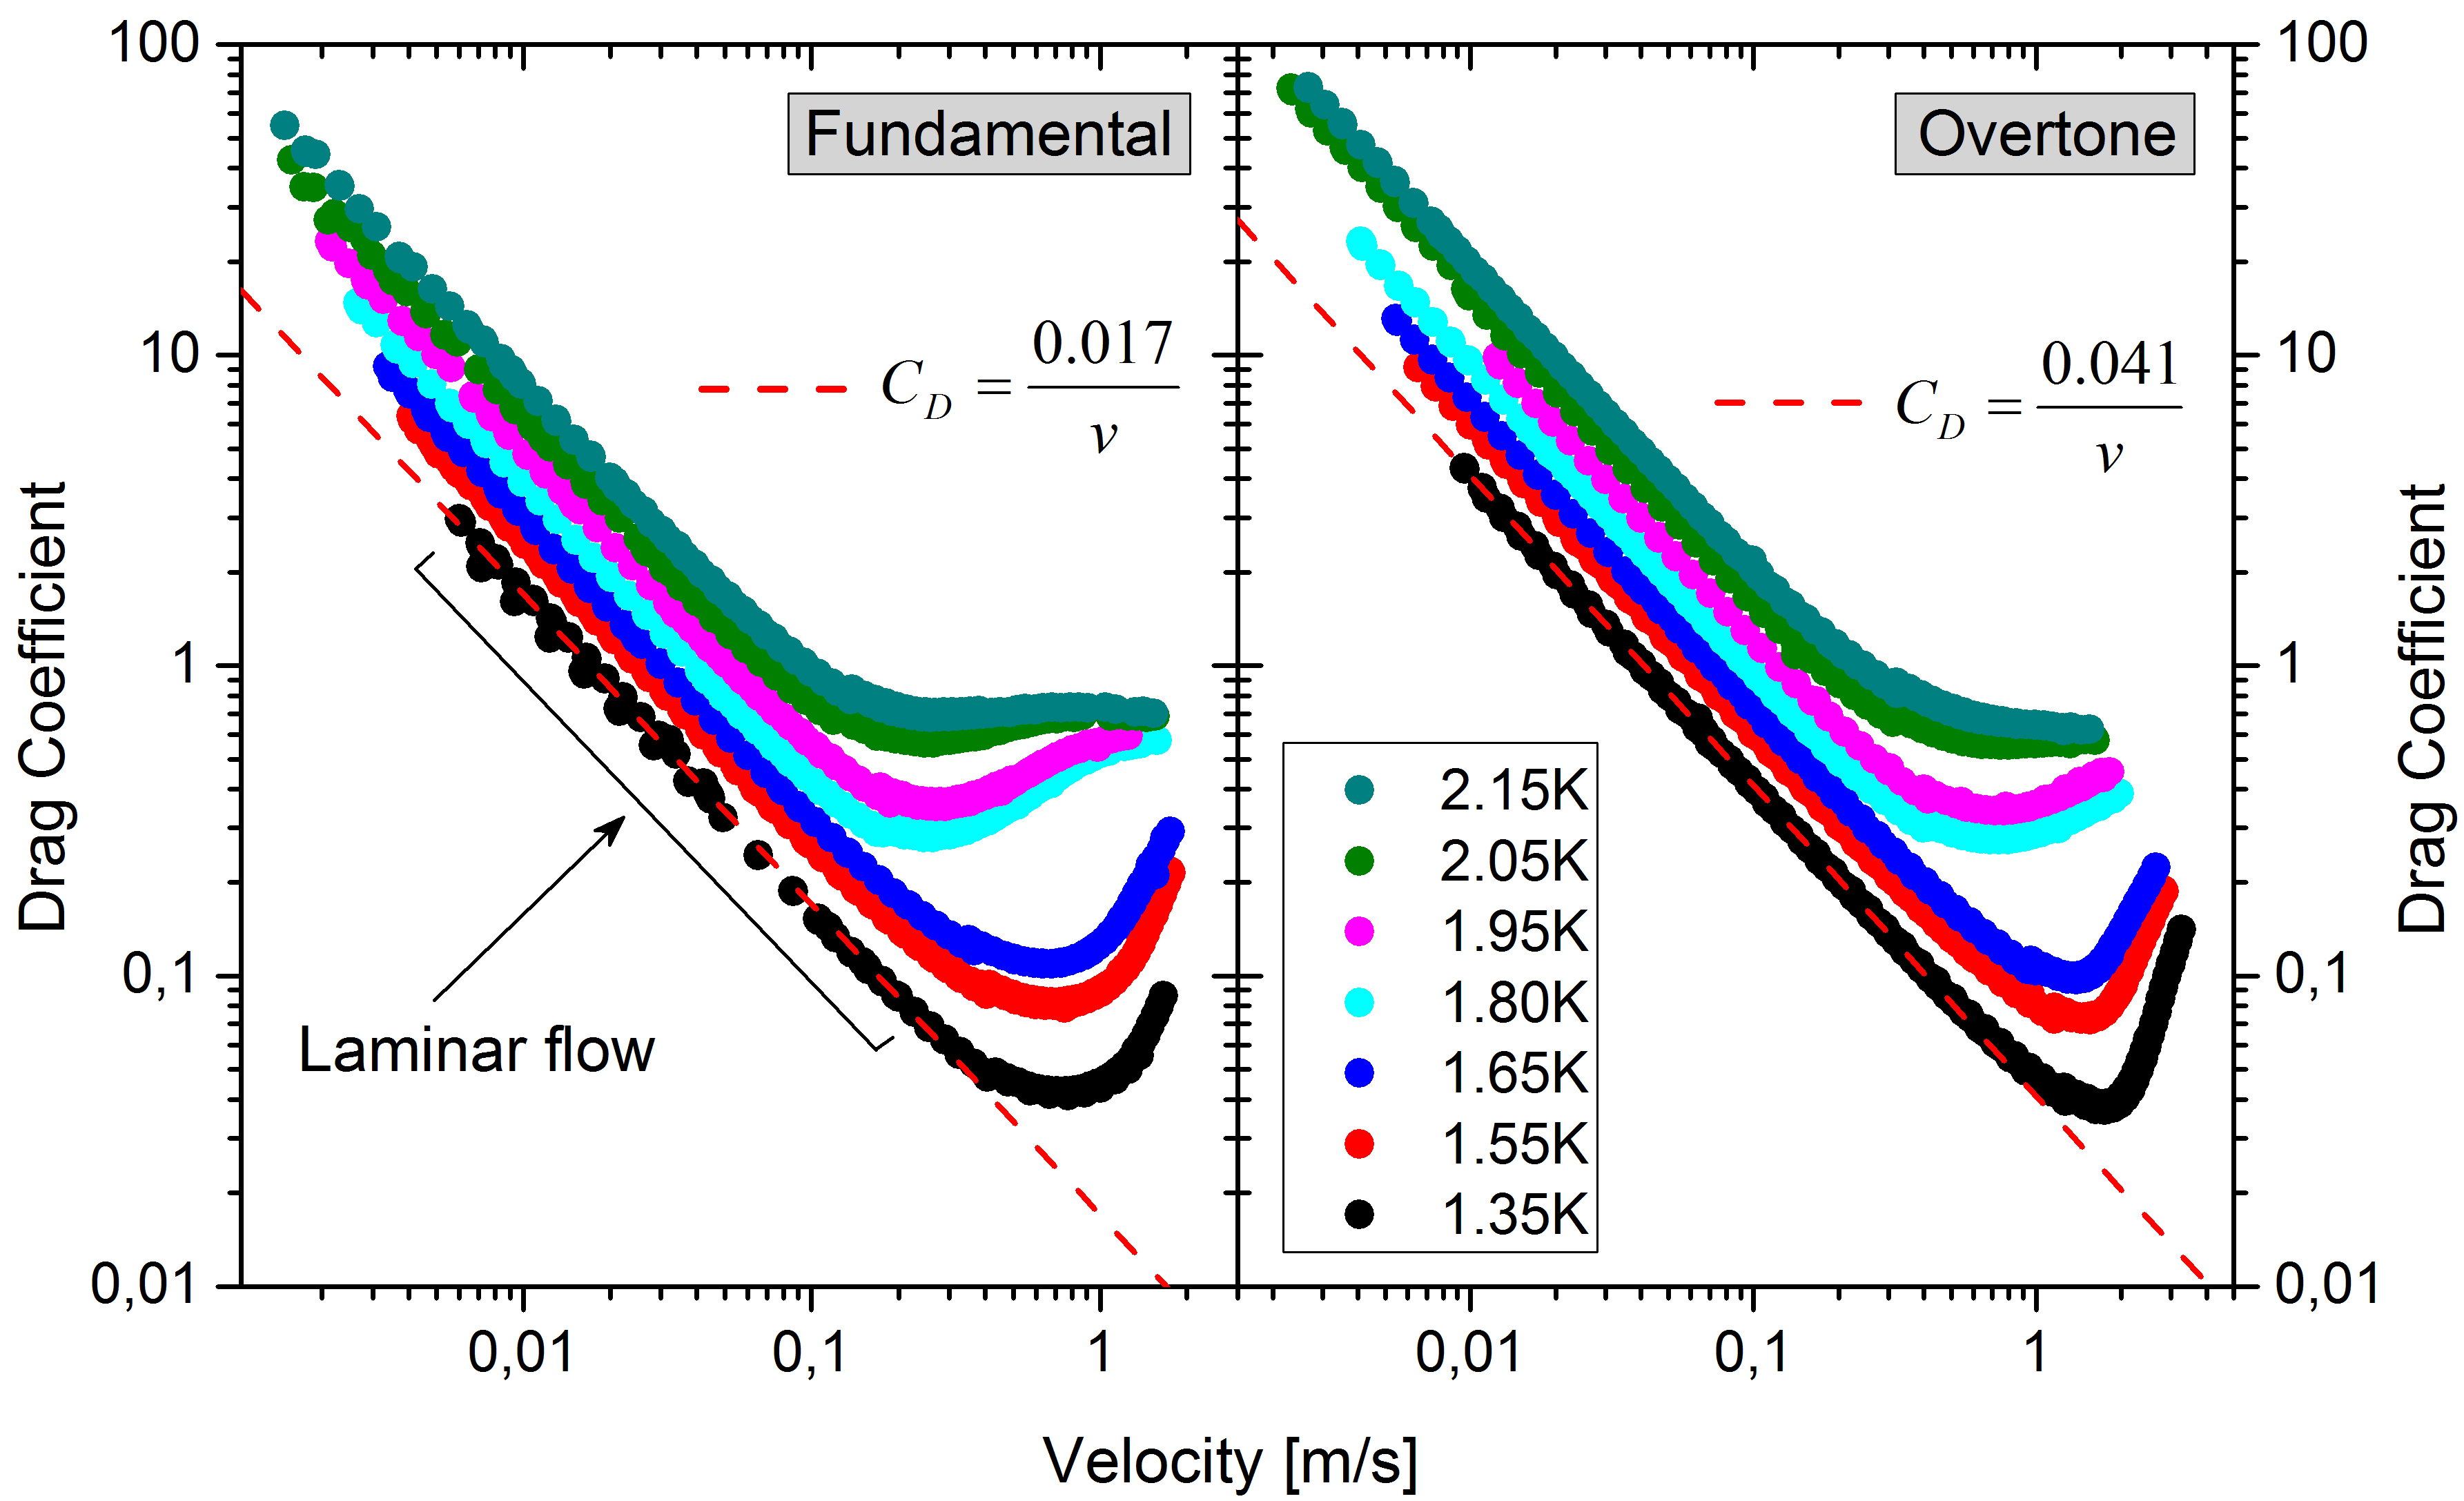
\includegraphics[width=1\textwidth]{graphs/Merged_C_v}
	\caption{Drag coefficients plotted against the peak velocity of the oscillating tuning fork. The \textit{red dotted lines} fit the laminar part of the dependences for the temperature $ 1.35\unit{K} $, with different values of the fitting parameter for the two tuning fork modes. }
\end{figure}

Looking at the graph in {\sffamily\textbf{Figure 3.6}} we can recognize ``two types'' of curves. Those for which the non-linearity seemingly appears at one certain velocity, and those for which the onset arises when exceeding different velocities. This can be regarded as the first sign that either quantum turbulence (QT) or classical turbulence (CT) may occur first under different conditions. Moreover, we note that the $ 2.15 \unit{K}$ curve seems to approach the dependence of the drag coefficient as we know it from classical fluids, with the limiting constant value not far below $ C_D = 1 $, which is expected for tuning forks in a classical fluid~\cite{PraguePRB}.

Within the two-fluid model, we distinguish between the drag coefficient and oscillatory Reynolds number for the whole fluid $ C_{D}$, $ \text{Re}_{\delta_{\ind n}} $ and only for the normal component alone $ C_{D{\ind n}} = 2F/S\rho_{\ind n}v^2 = C_D \rho/\rho_{\ind n} $, $ \text{Re}_{\delta_{\ind n}} = v\rho_{\ind n}\delta_{\ind n}/\eta_{\ind n} $. For each temperature, the values for the density of normal component $ \rho_{\ind n} $ and dynamical viscosity were taken from \cite{donnelly}.

The resulting graph ({\sffamily\textbf{Figure 3.7}}) showcases three interesting and important facts. First, within the laminar range, all curves collapse to a single dependence, confirming the validity of the scaling proposed in {\sffamily\textbf{Sections 3.3, 3.4}} and establishing the oscillatory Reynolds number as a suitable dimensionless parameter. Second, for both modes, the laminar part could be fit by the exact same straight line. This represents the fact that the drag force scaling in the high-frequency regime is, with all likelihood, independent on the velocity profile along the prong and holds even for frequencies differing by a factor of $40\,000/6380\approx 6.27 $. Finally, the critical Reynolds number for generating classical turbulence within both fork modes (the $ 2.15\unit{K} $ curve best shows) has been estimated as $ \text{Re}_{\delta_{\ind n}c}=7\pm 2 $.




\begin{figure}[h!]
	\centering
	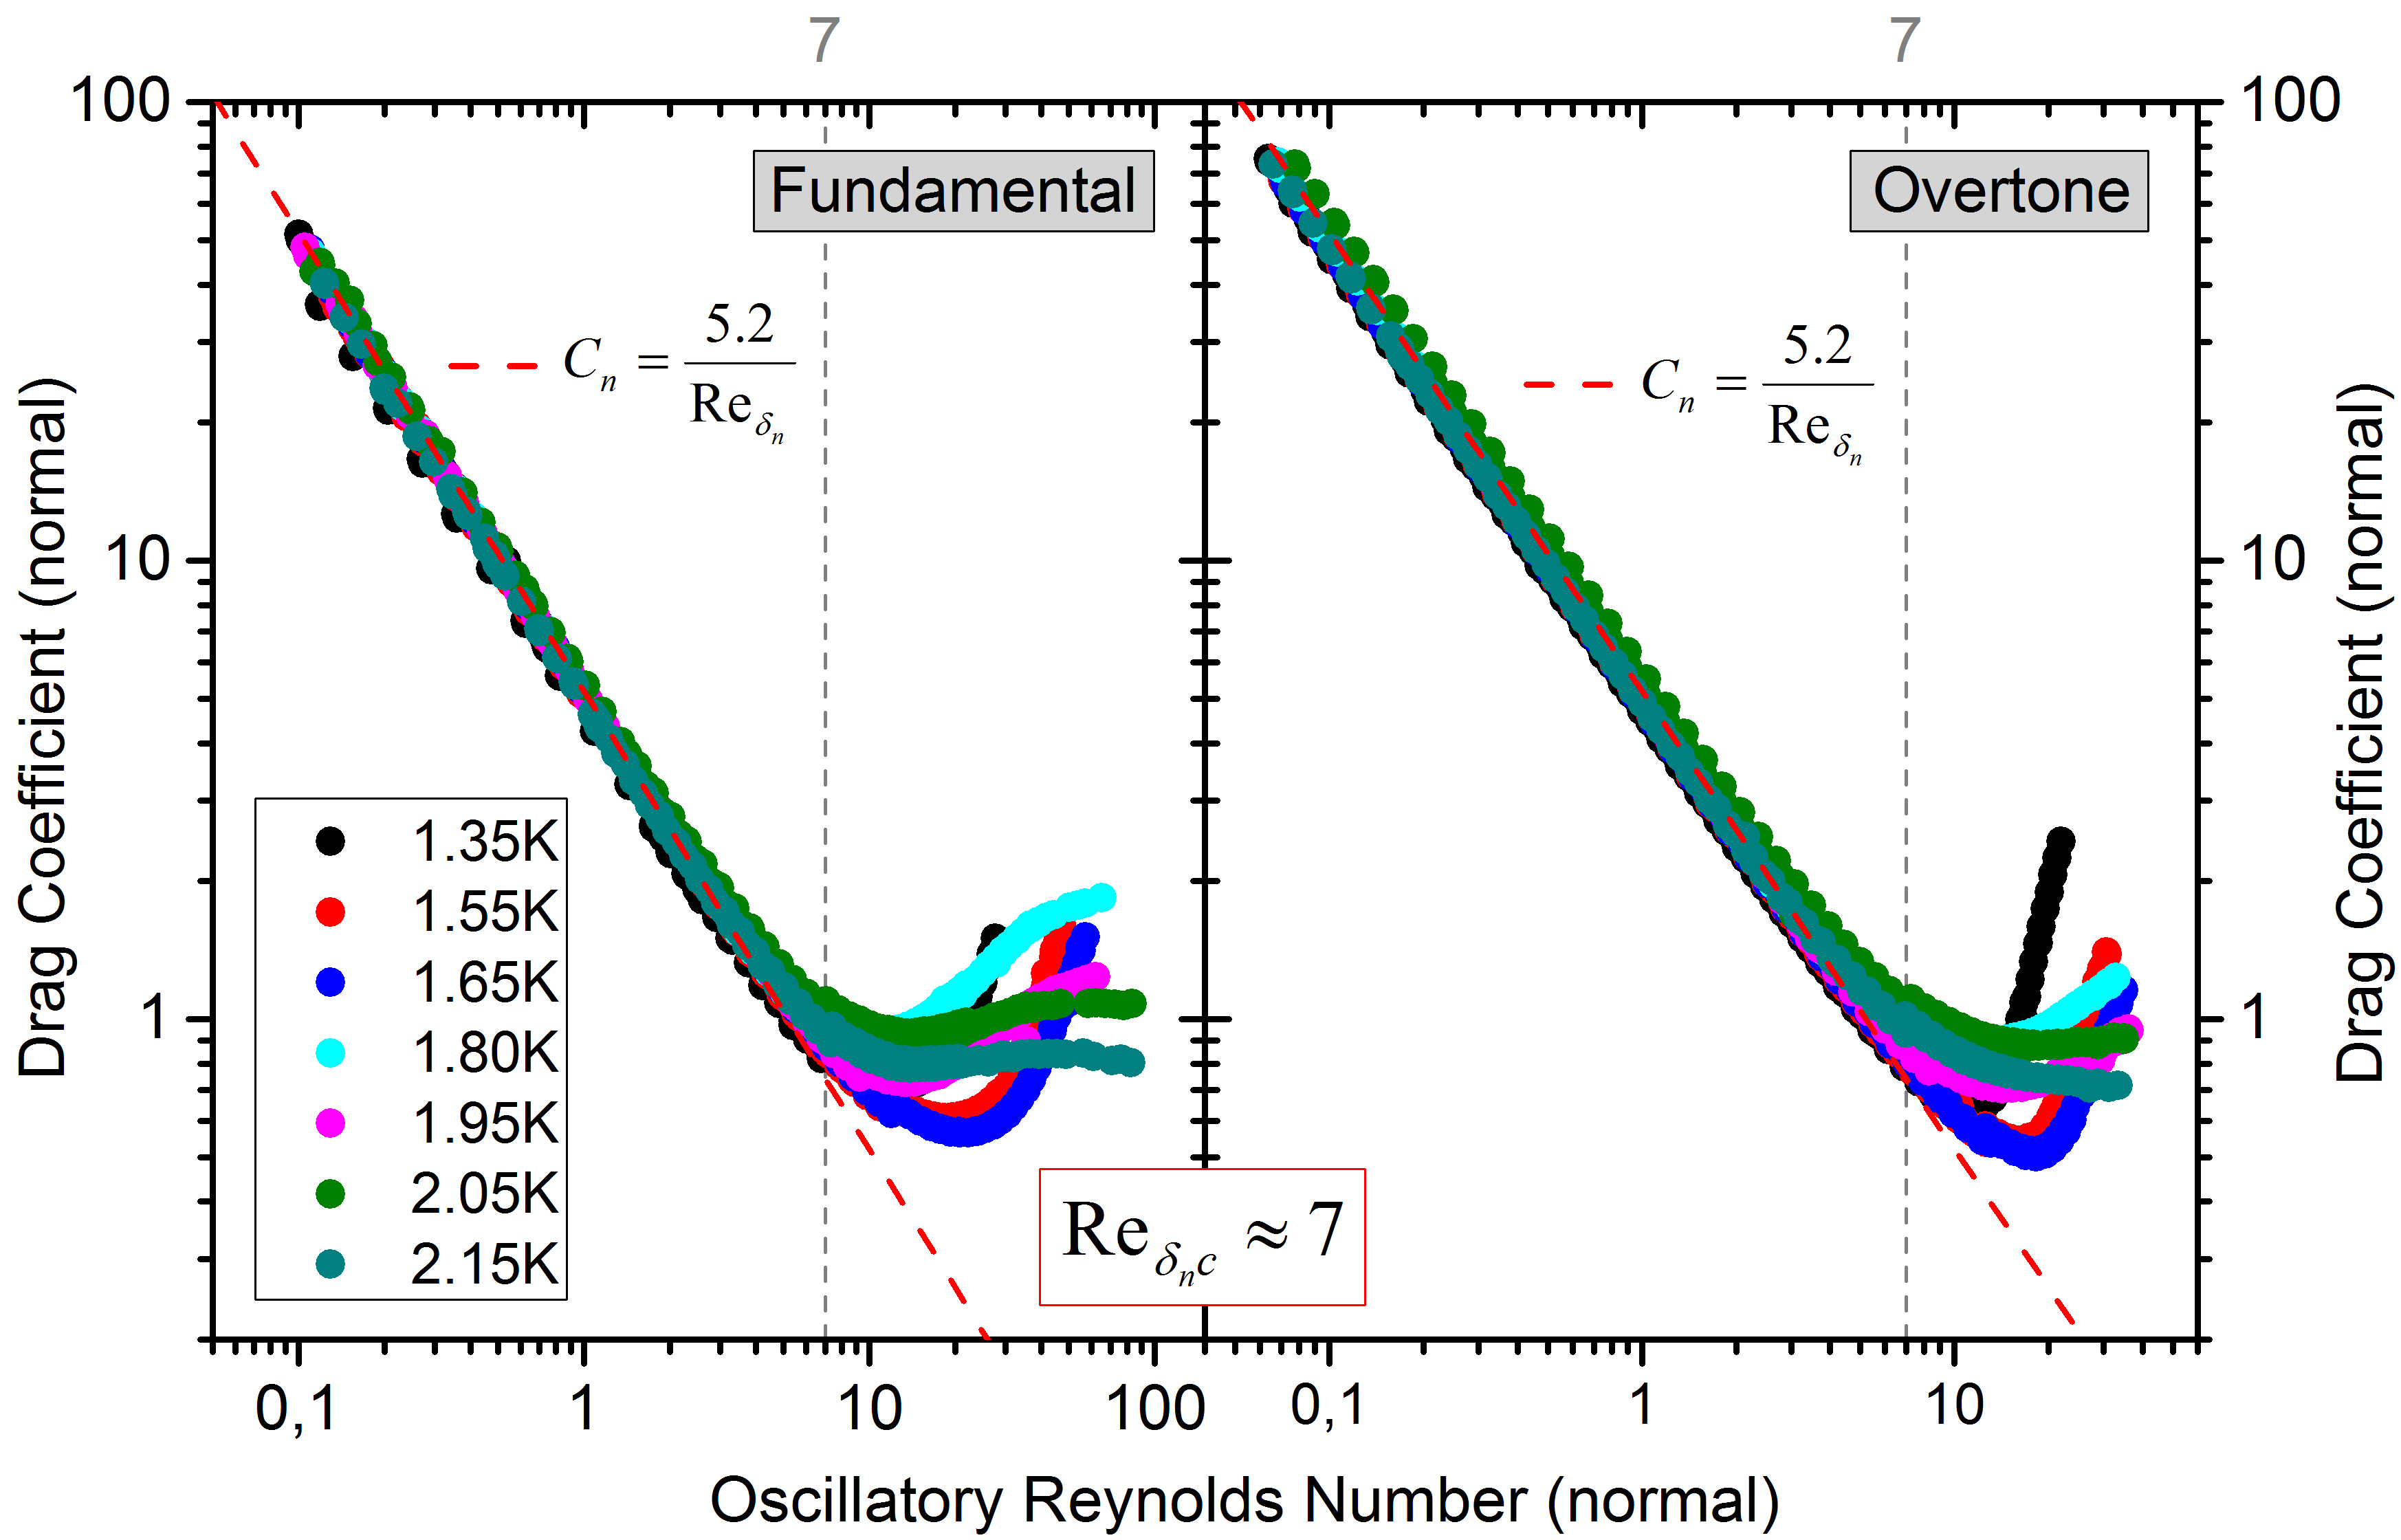
\includegraphics[width=1\textwidth]{graphs/Merged_Cn_Ren}
	\caption{Drag coefficient plotted against the oscillatory Reynolds number, both evaluated for the normal component alone. Statistically, the onset of non-linear drag occurs for all temperature curves within the interval $ \text{Re}_{\delta_{\ind n}}^{\ind{crit}}=7\pm 2 $. The presented data are, however, affected by the observed unsystematic behaviour of the tuning forks with regard to the onset of non-linear drag, as discussed in the accompanying text. The \textit{red dotted line} shows the fit of the laminar regime, which is exactly the same for both modes.}
\end{figure}

At this point, we have to remind the reader that during the actual experiment, we have observed unsystematic behaviour of the tuning forks and therefore the data shown here is very likely affected by this issue. In drag force measurements, this manifested in such a manner that the onset of non-linear drag occurred at different values of $ \text{Re}_{\delta_{\ind n}} $ when the same temperature was studied at different points during the entire experiment. Therefore, the estimated critical value of $ \text{Re}_{\delta_{\ind n}c}=7\pm 2 $ ought to be taken with some reservations, as it corresponds only to a subset of the acquired data (the four higher temperatures), for which we have reasonable grounds to claim that no significant change of the tuning fork behaviour occurred in between the measurements. Nevertheless, the actual critical value (incorrect as it may be) has little bearing on the interpretation presented below, and we choose to use this particular value as it still describes the majority of the data with a good degree of accuracy.

\section{Correlation of Results}


In the following, we connect the results of vortex line density measurement and a non-linear behaviour of drag coefficient. We will be able to distinguish between quantum turbulence (QT), caused by the presence of quantized vortices and classical-like turbulence (CT) of the normal component. Within this Section, we work only with the fundamental mode.


\begin{figure}[h!]
	\centering
	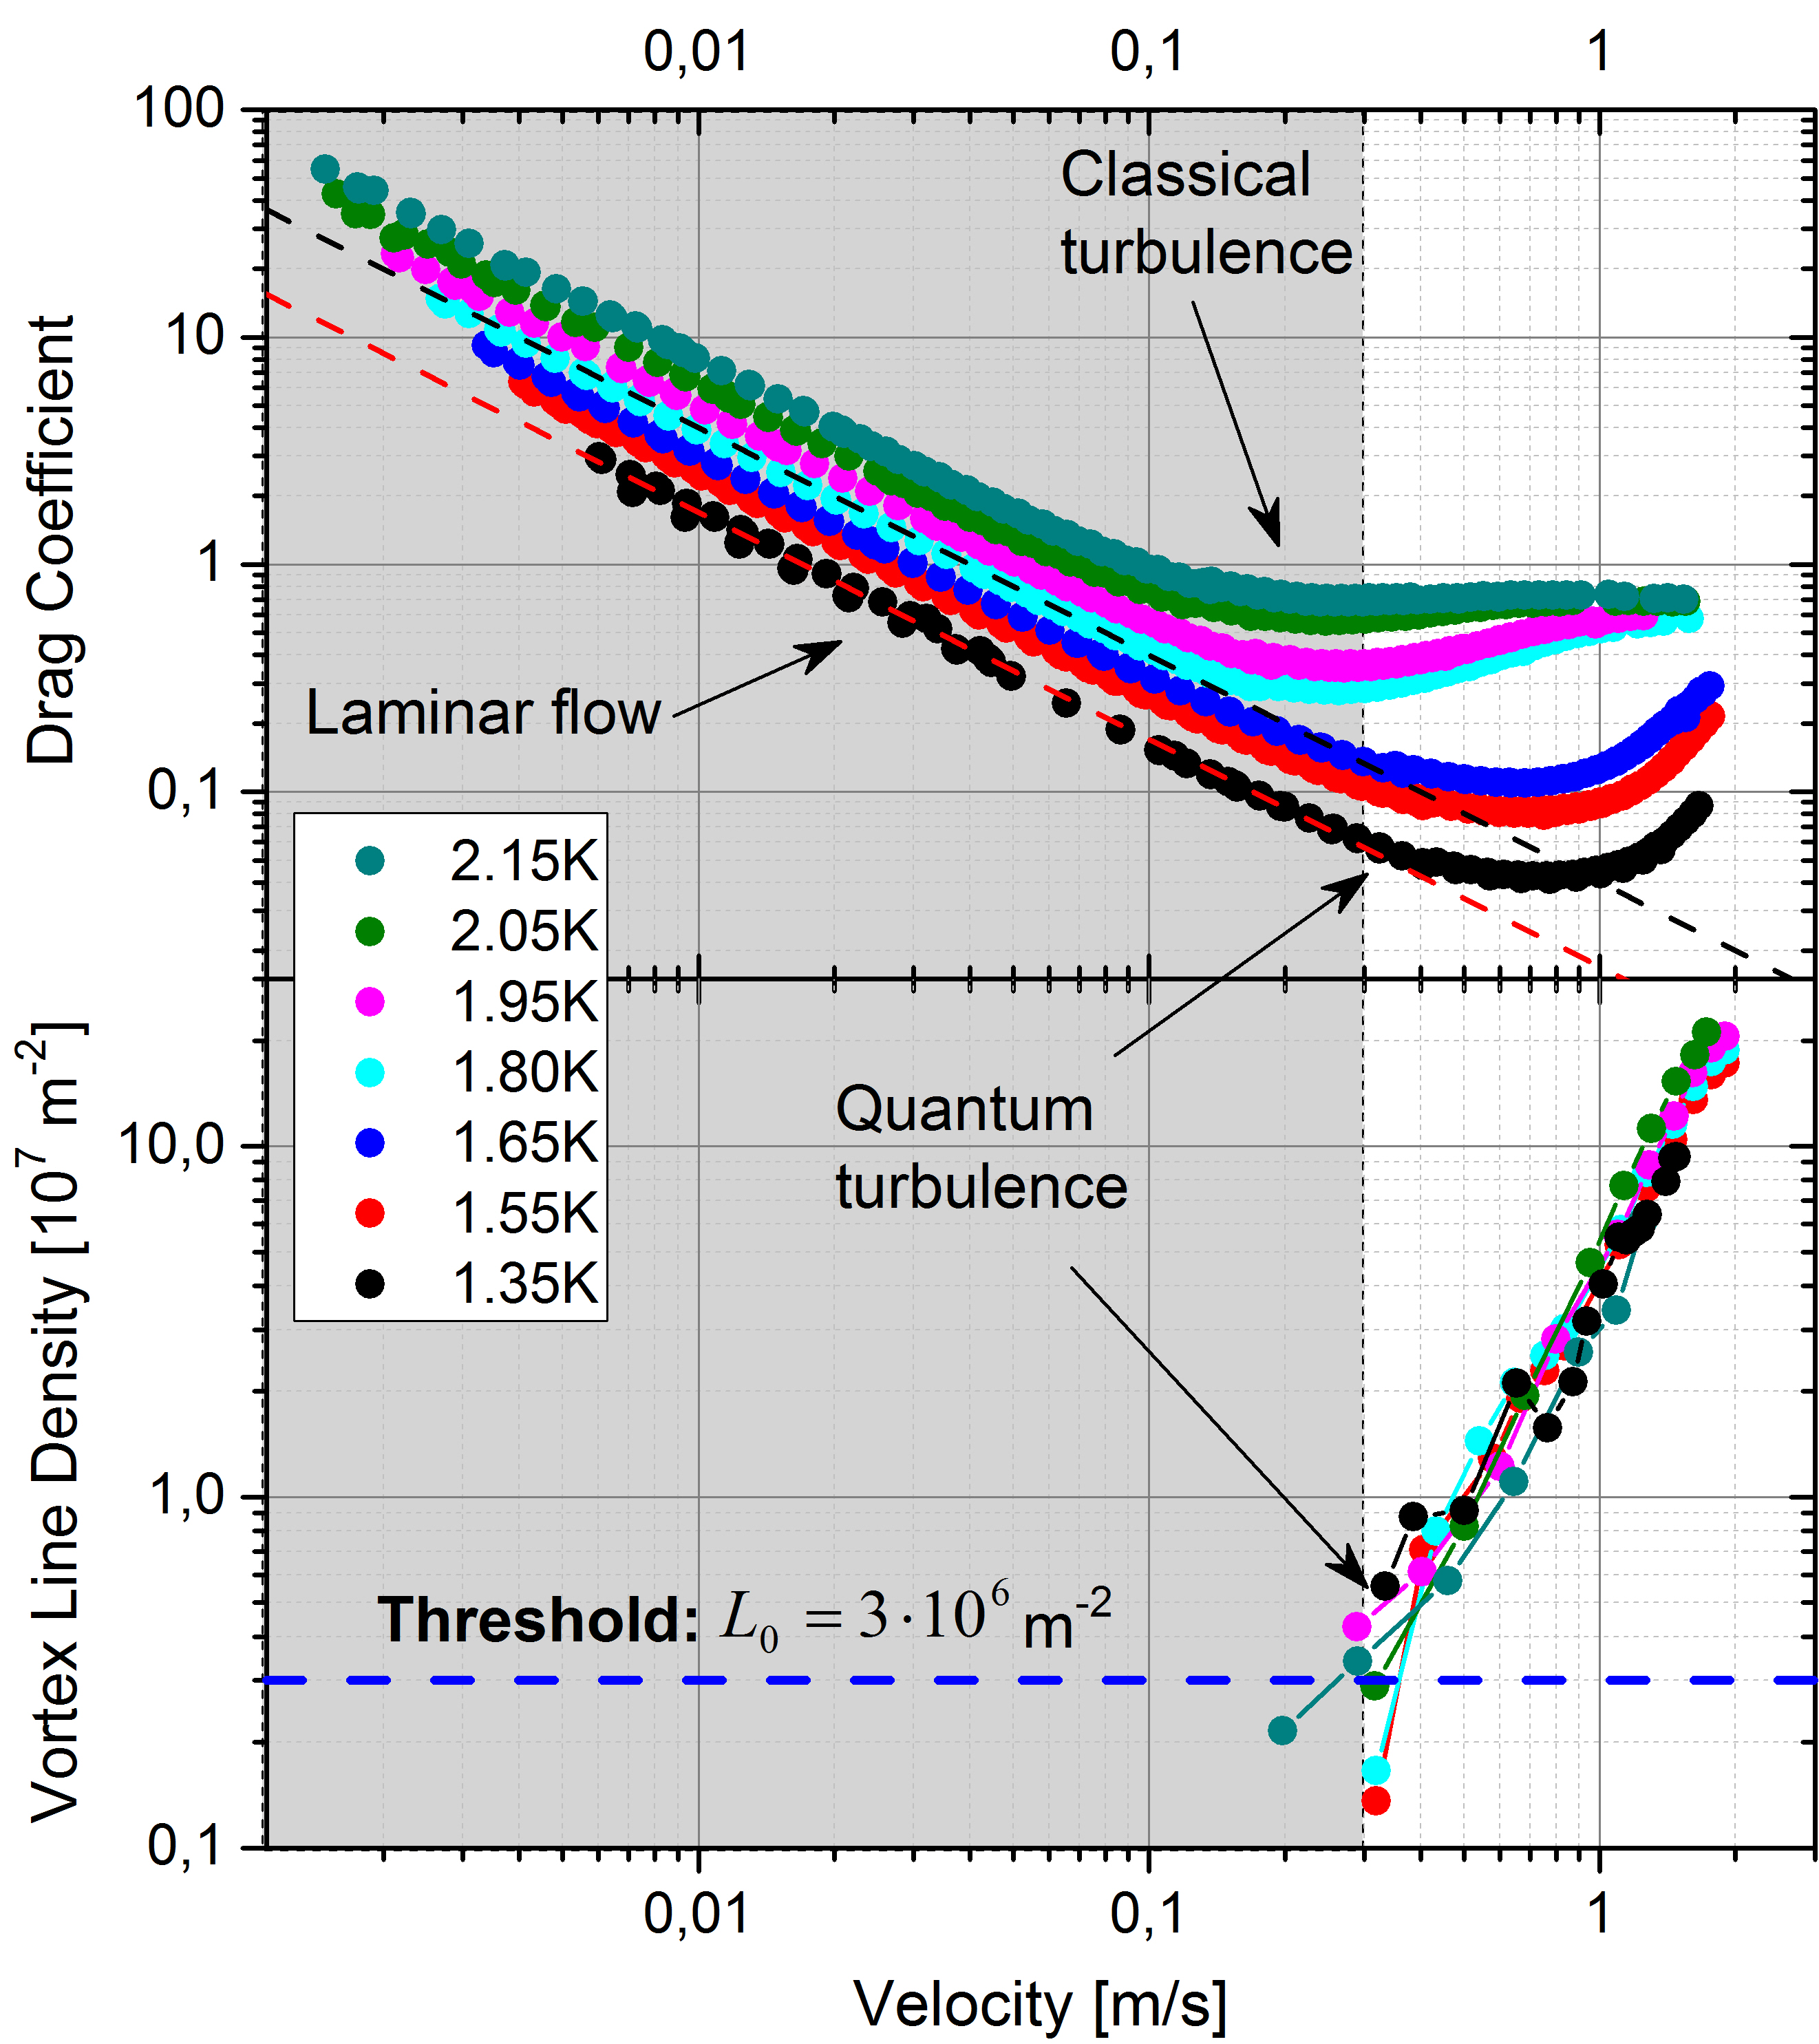
\includegraphics[width=0.8\textwidth]{graphs/Merged_C+L_fund}
	\caption{Velocity dependence of drag coefficient $ C_D $ and vortex line density $ L $ for the fundamental mode of the tuning fork. The \textit{blue, red and black dotted lines} are the threshold level and laminar drag fits for $ 1.35\unit{K} $ and $ 1.80\unit{K} $ curves, respectively. The \textit{shaded zone} marks sub-critical velocities from the point of view of detection of quantized vortices by second sound, and corresponds to the laminar drag regime for the lowest three temperatures.}
\end{figure}


In {\sffamily\textbf{Figure 3.8}} we clearly see the correlation between the production of QT (lower graph) and the onset of non-linear drag force in $ 1.35\unit{K} $, $ 1.55\unit{K} $ and $ 1.65\unit{K} $ curves. For the rest of curves ($ 1.80 \unit{K} $ and above), the density of normal component is much higher and consequently the critical oscillatory Reynolds number was exceeded earlier than the critical velocity $v_{\ind{c}}^{\ind f}$.

However, from {\sffamily\textbf{Figure 3.8}} we are not sure, whether QT really occurred first or CT was just too weak to be noticed by our devices. The graphs in {\sffamily\textbf{Figure 3.9}} compare the normal drag coefficient $ C_{D\ind{n}} $ and vortex line density $ L $ against $ \text{Re}_{\delta_{\ind n}} $ and better illustrate the situation. We purposely zoomed the region near transition. 


\begin{figure}[h!]
	\centering
	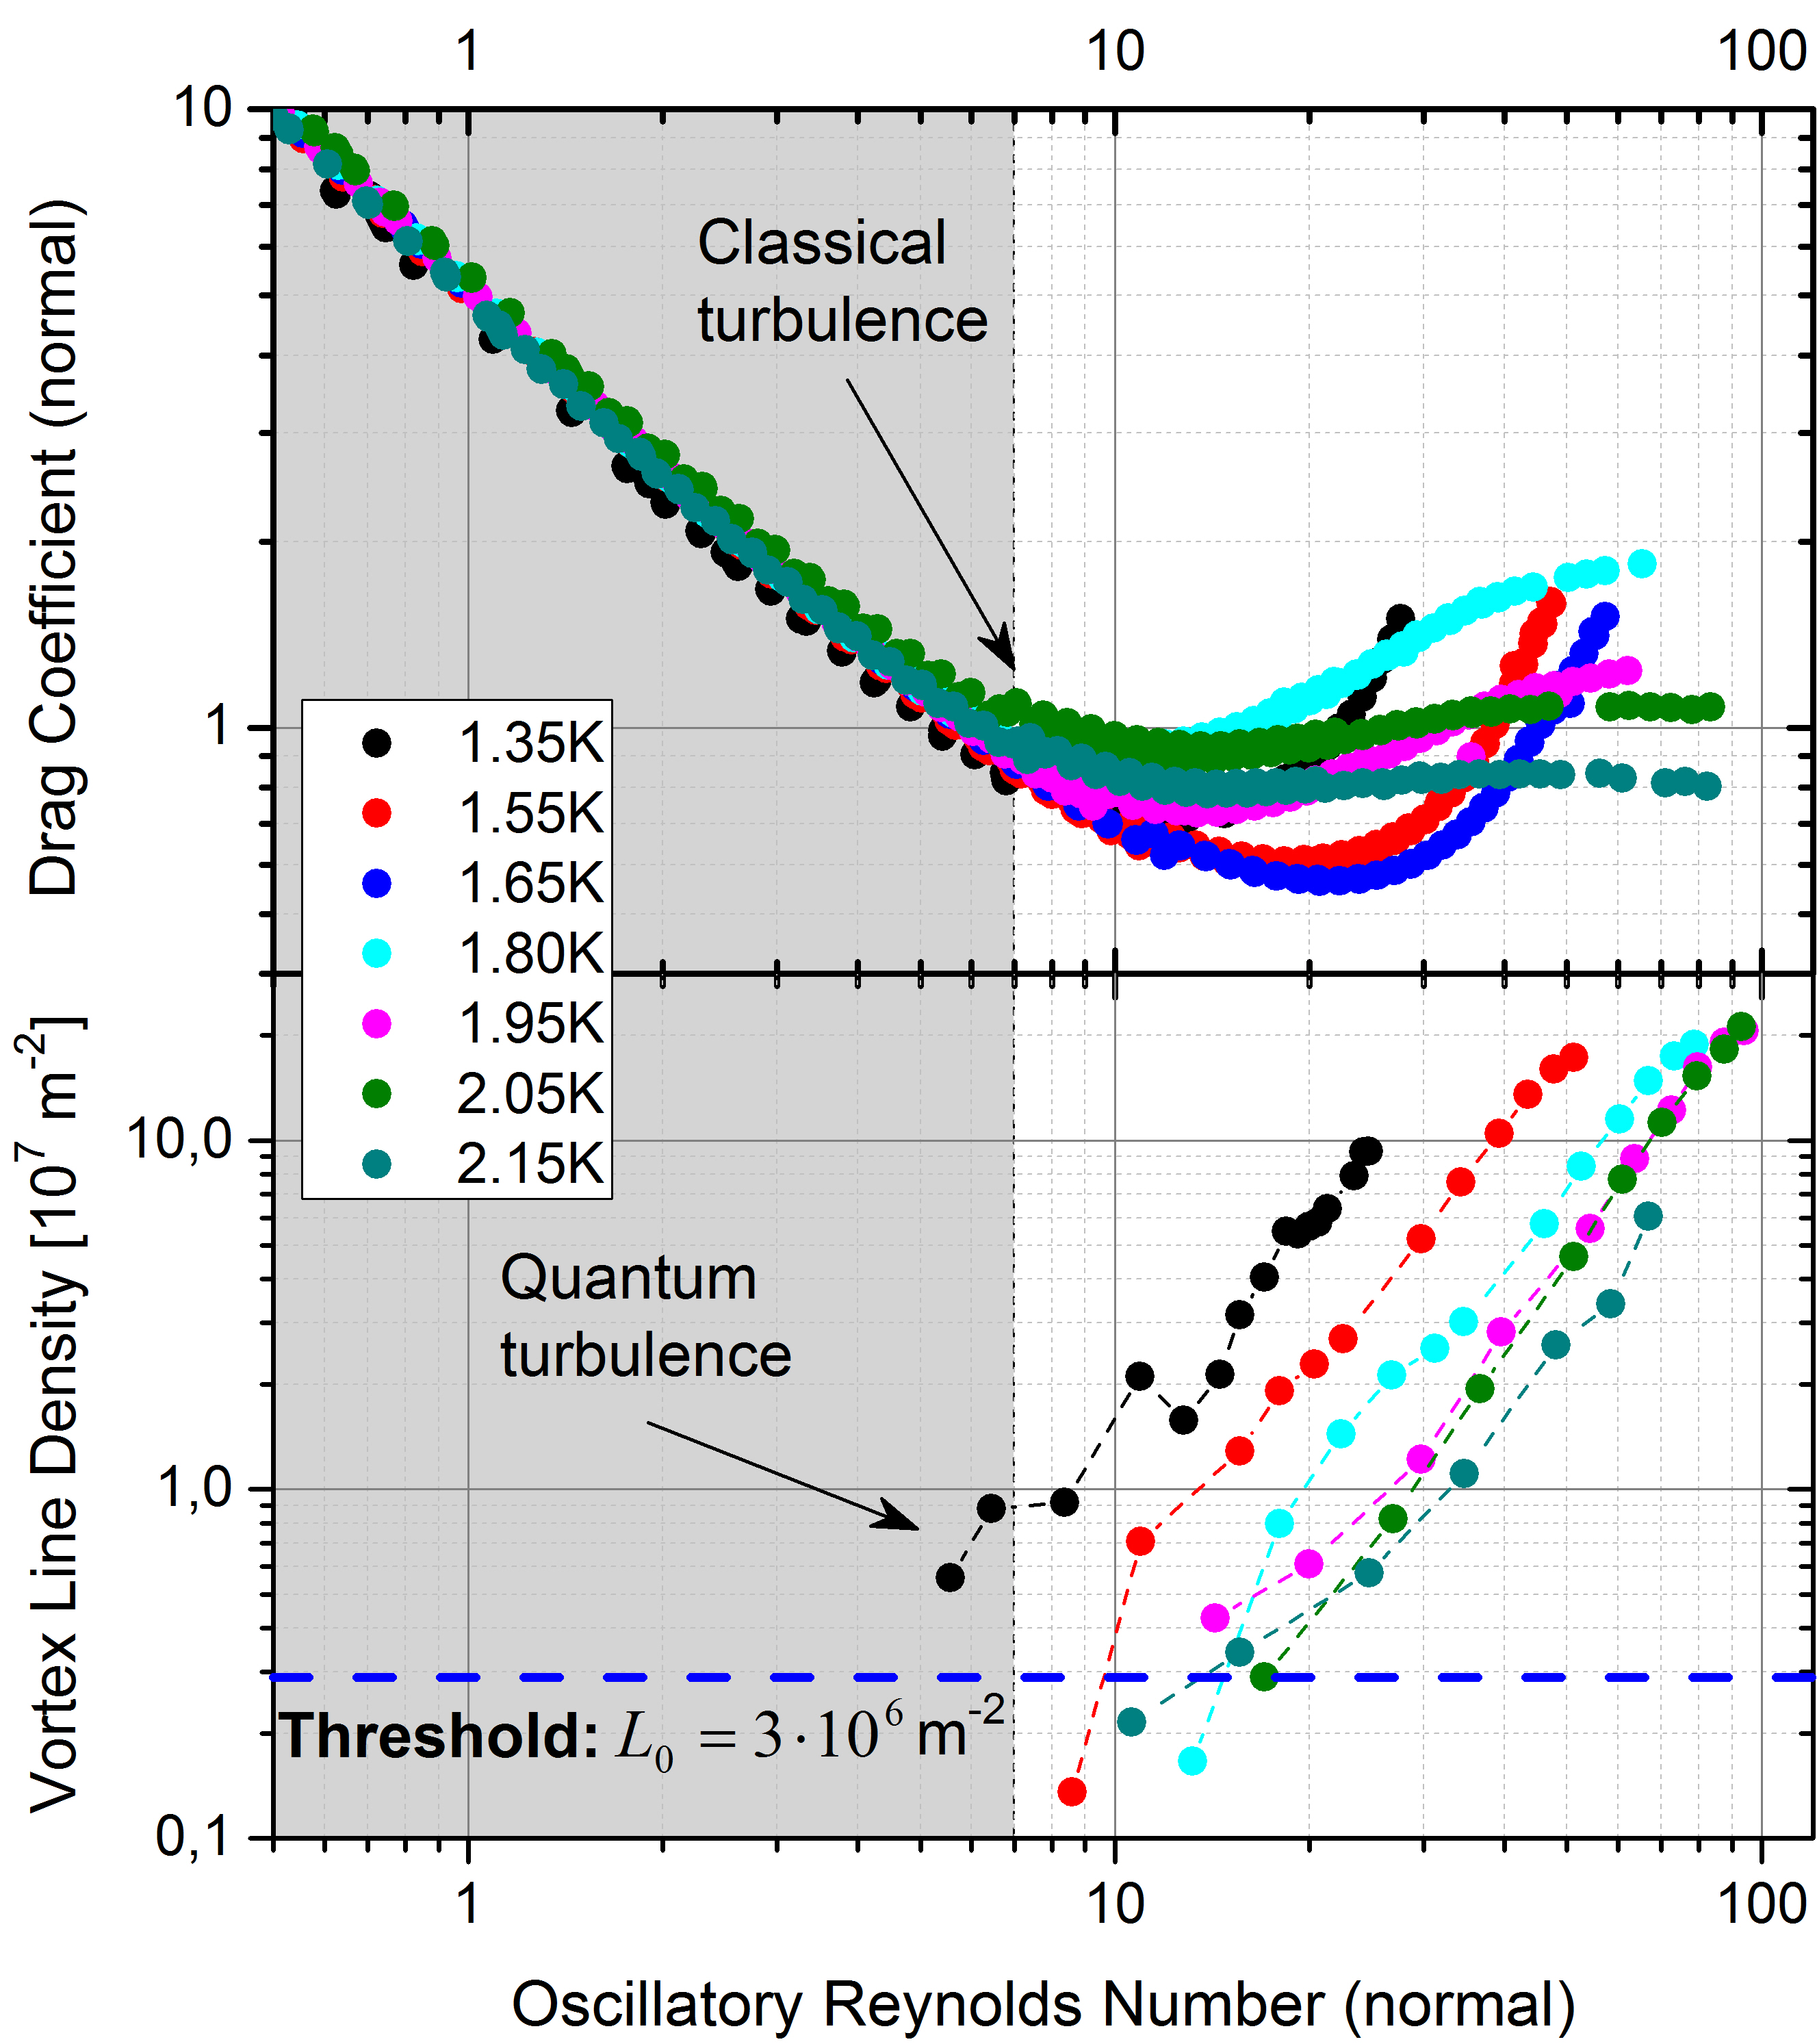
\includegraphics[width=0.8\textwidth]{graphs/Merged_C+L_Ren_fund}
	\caption{Plot of the normal fluid drag coefficient $ C_{D\ind{n}} $ and vortex line density $ L $ against the oscillatory Reynolds number $ \text{Re}_{\delta_{\ind n}} $ for the fundamental mode of tuning fork.}
\end{figure}

As shown before, classical turbulence of the normal component arises roughly when exceeding the critical $ \text{Re}_{\delta_{\ind n}c} \approx 7$. On the other hand, QT has been detected above $ v_{\ind{c}}^{\ind{f}} \approx 0.3 \unit{m/s}$, so in {\sffamily\textbf{Figure 3.9}} it is clearly shown that a considerable QT was detected as first only for temperature $ 1.35 \unit{K} $. However, following the previous set of graphs in {\sffamily\textbf{Figure 3.8}}, we came to a similar conclusion for all three of the lowest temperatures ($ 1.35 \unit{K} $, $ 1.55 \unit{K} $, $ 1.65 \unit{K} $), not just the lowest one. This could be understood in such a manner that although CT could have occurred first for $ 1.55 \unit{K} $ and $ 1.65 \unit{K} $, QT followed shortly and soon became a dominant contribution to the drag force due to the high density of the superfluid component.

\newpage


\subsection*{Overtone Mode}

Here we perform exactly the same dependencies and similar conclusions we introduced for the fundamental mode in previous {\sffamily\textbf{Section 3.3}}.

\begin{figure}[h!]
	\centering
	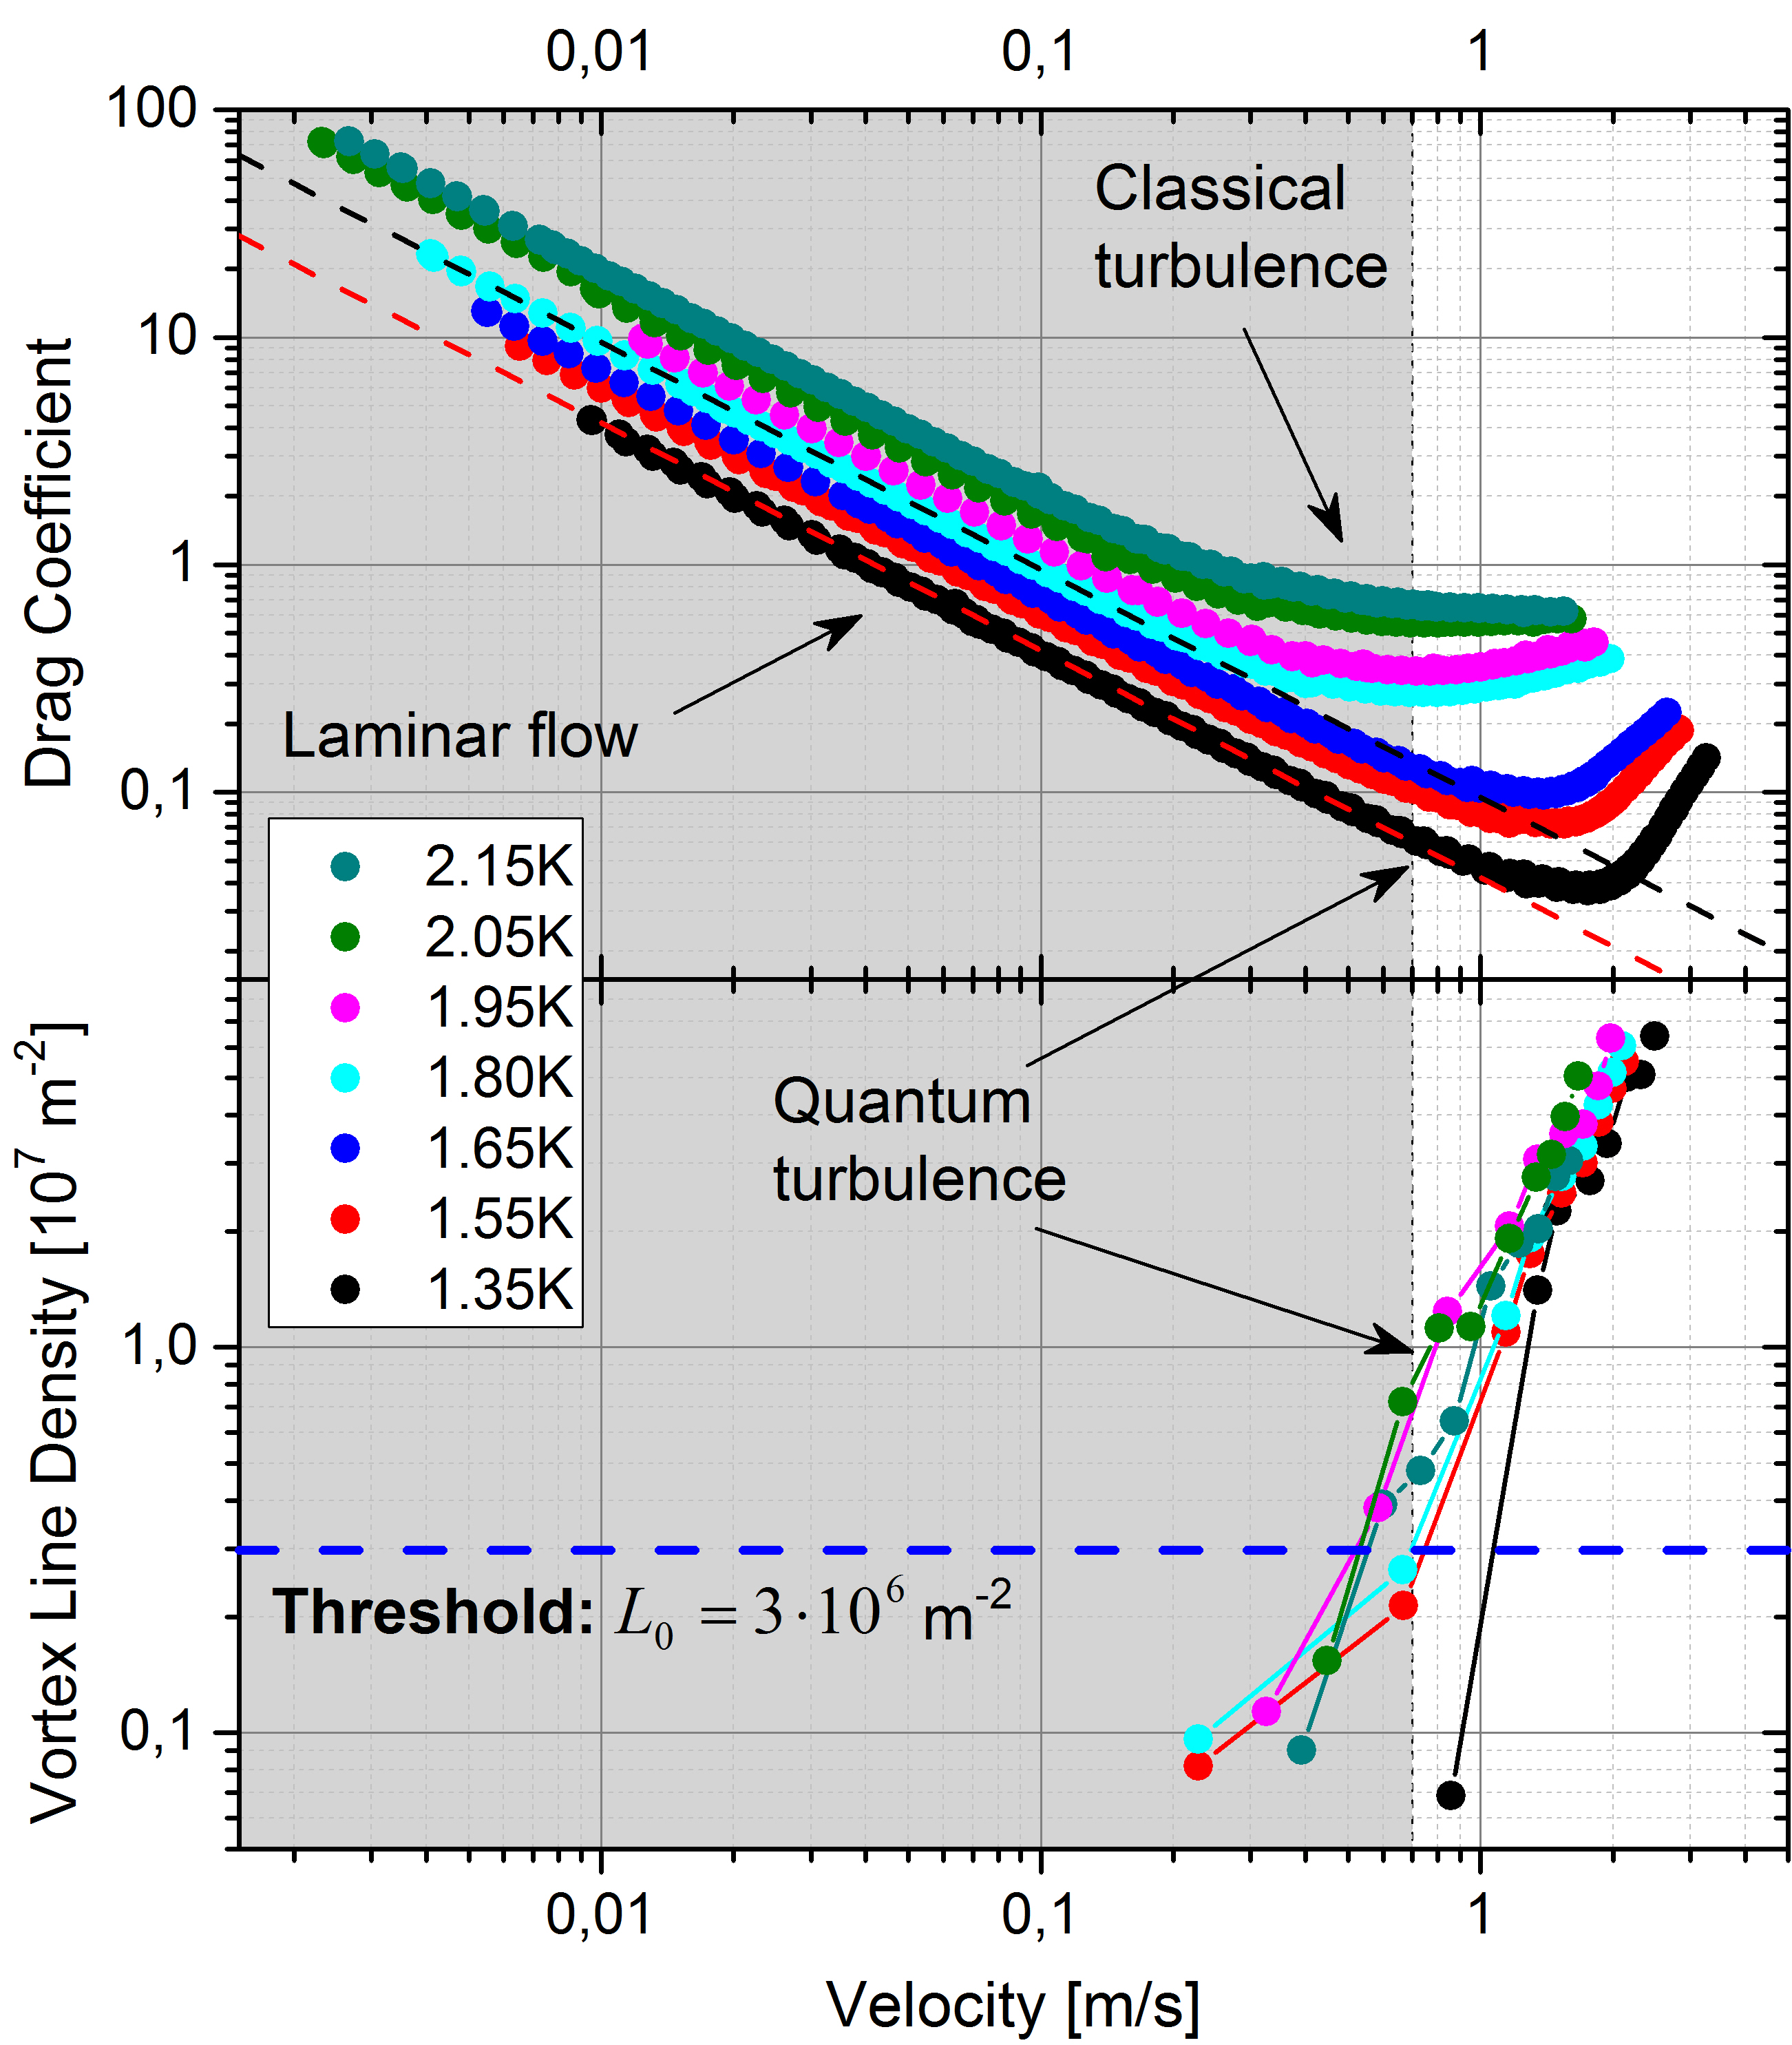
\includegraphics[width=0.8\textwidth]{graphs/Merged_C+L_over}
	\caption{Velocity dependence of drag coefficient $ C_D $ and vortex line density $ L $ for the overtone mode of the tuning fork. The \textit{blue, red and black dotted lines} are the threshold level and laminar drag fits for the $ 1.35\unit{K} $ and $ 1.80\unit{K} $ curves, respectively. The \textit{shaded zone} marks sub-critical velocities from the point of view of detection of quantized vortices by second sound, and corresponds to the laminar drag regime for the lowest three temperatures.}
\end{figure}

The situation in overtone mode seemingly does not differ from the case of fundamental - the only difference is that the correlation of QT formation and onset of non-linear drag is harder to see by an eye.

The plots of $ C_{D\ind{n}} $ and $ L $ against $ \text{Re}_{\delta_{\ind n}} $ (shown in {\sffamily\textbf{Figure 3.11}}) will help to illustrate the order in which the turbulence transitions likely occurred.


\newpage

\begin{figure}[h!]
	\centering
	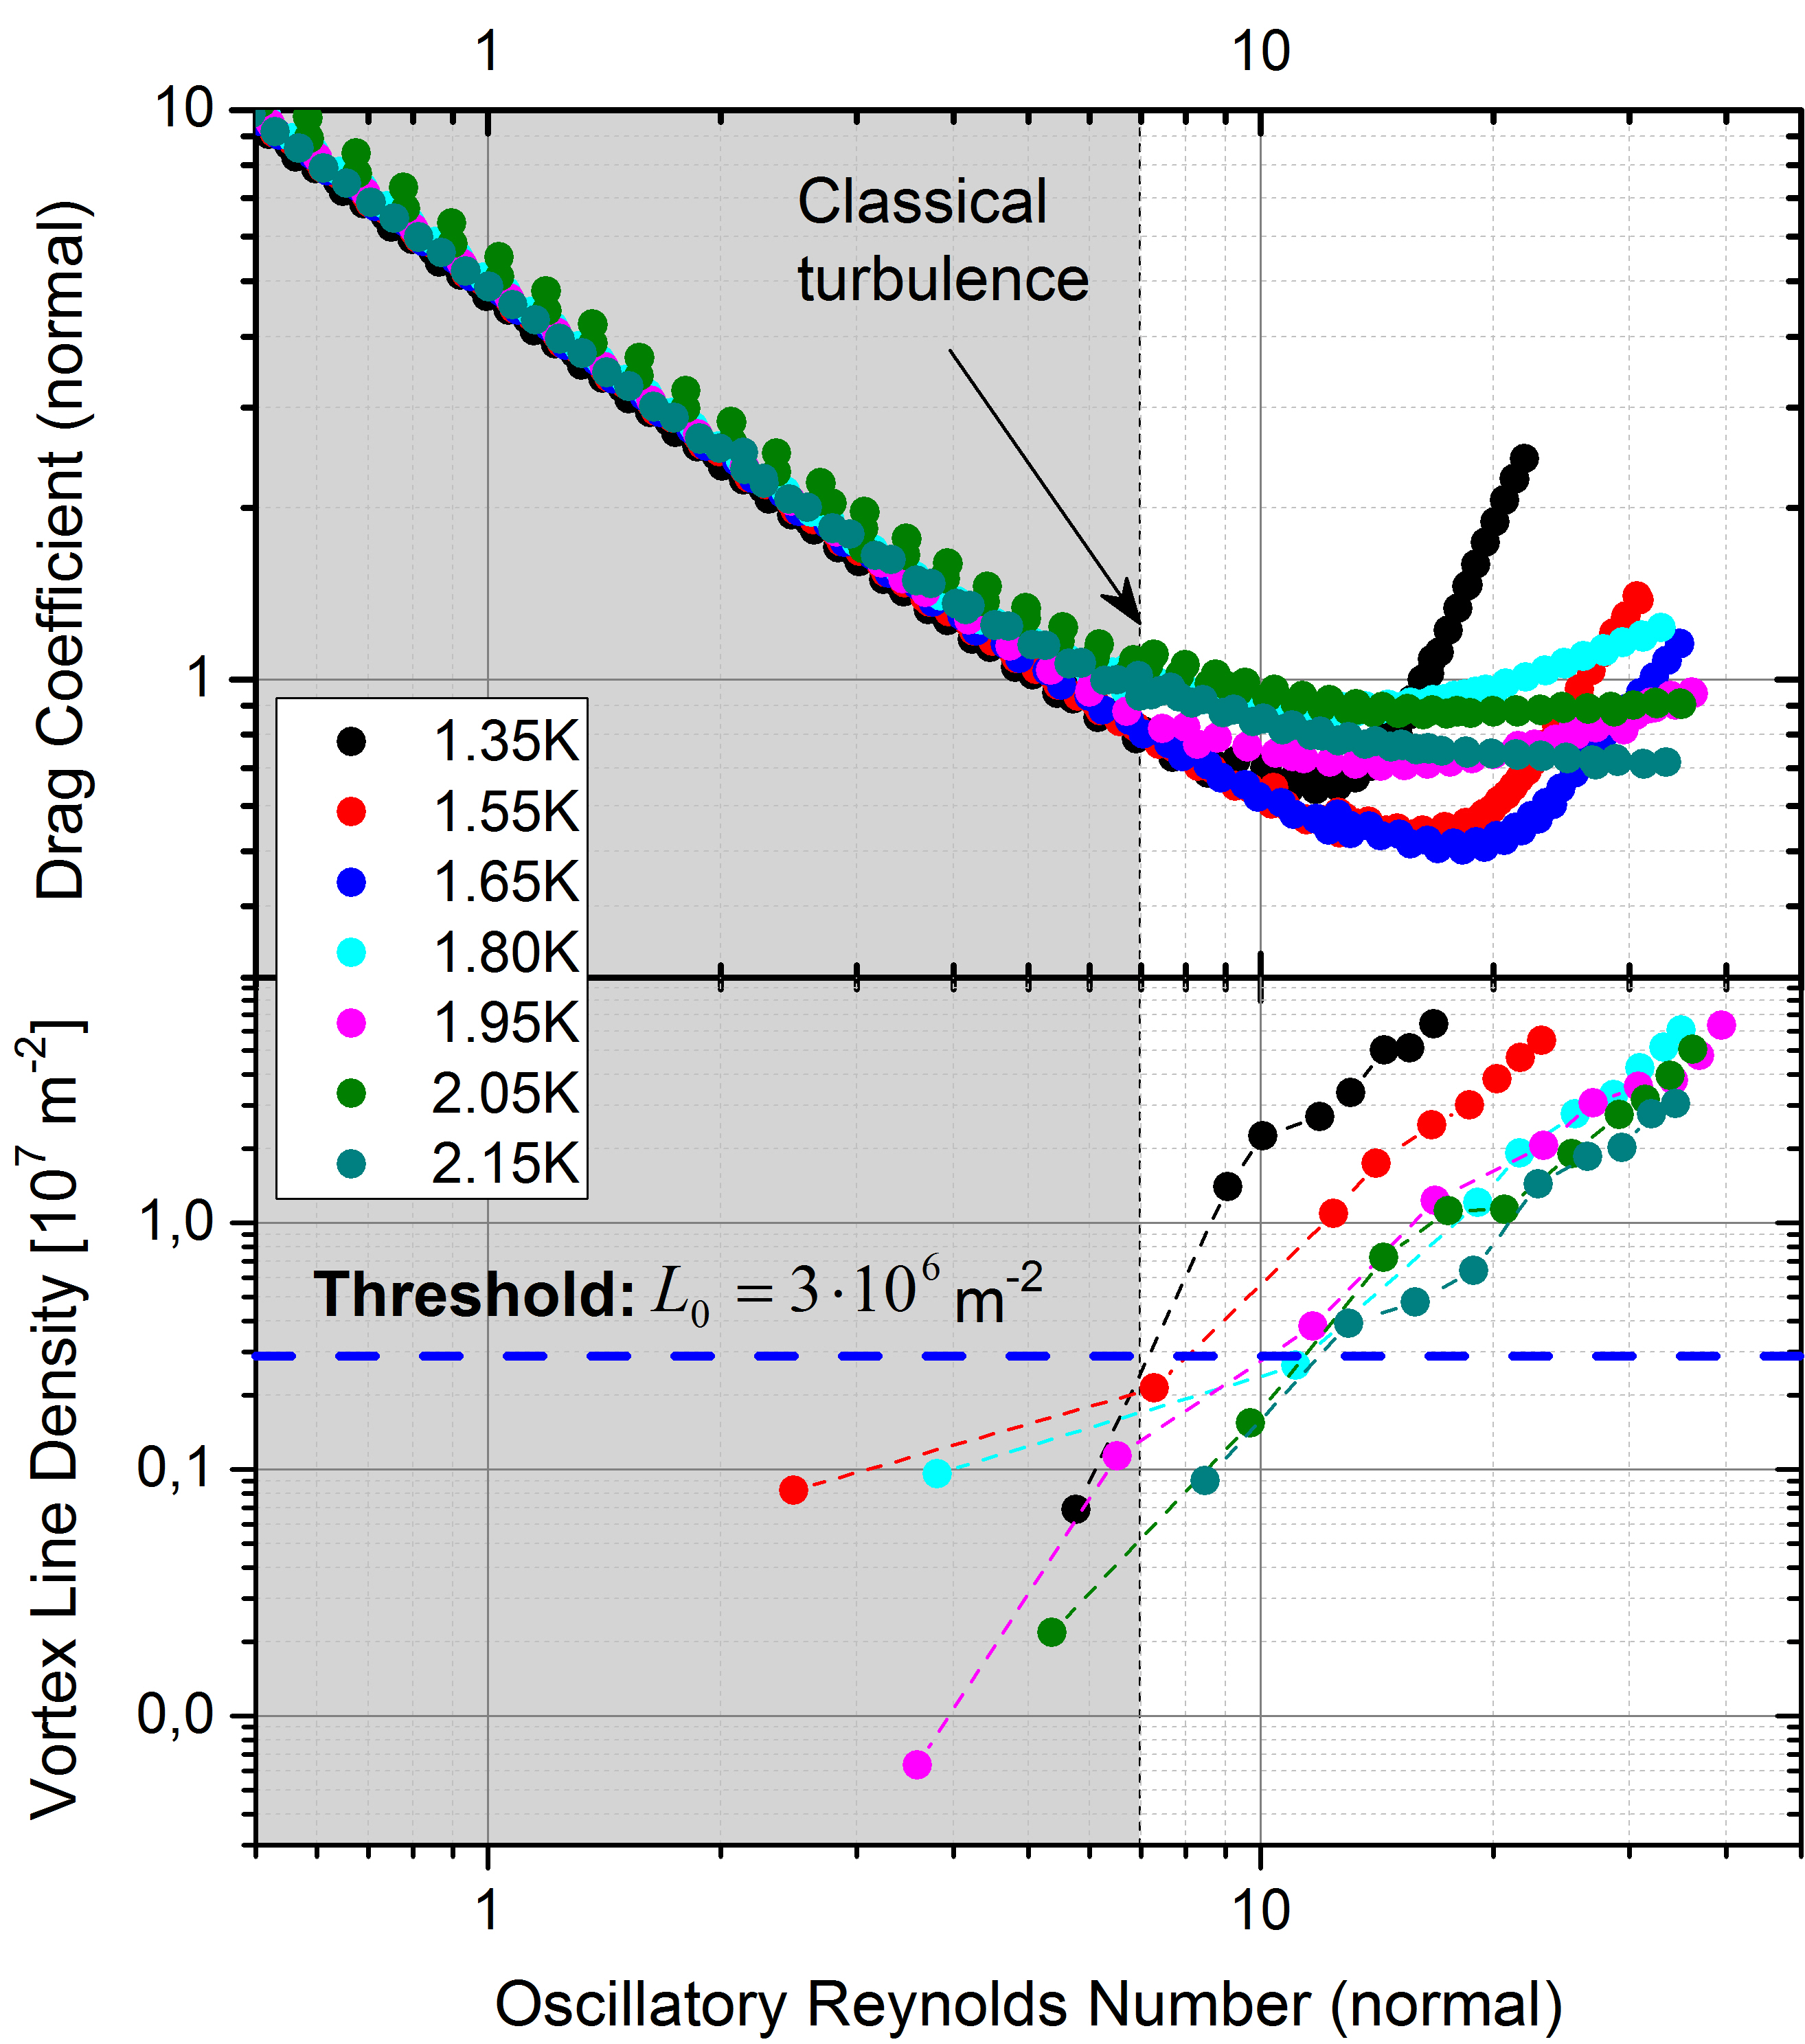
\includegraphics[width=0.8\textwidth]{graphs/Merged_C+L_Ren_over}
	\caption{Plot of the normal drag coefficient $ C_{D\ind{n}} $ and vortex line density $ L $ against the oscillatory Reynolds number $ \text{Re}_{\delta_{\ind n}} $ for the overtone mode.}
\end{figure}

In contrast with the fundamental mode, here QT did not occur earlier than CT at any of the shown temperatures. Although the graph in {\sffamily\textbf{Figure 3.10}} looked like the displayed non-linearities of the lowest three temperature curves are caused due to the formation of quantized vortices, this does not necessarily have to be true. As for the fundamental mode, CT may have appeared earlier, but QT dominated rapidly and hence CT could not be seen in the drag coefficients reliably.

\newpage

\section{Discussion}

In this Section we summarize all the observations and found relations between the measured drag forces and the vortex line densities detected by second sound attenuation. We also perform the \textit{flow phase diagram} for better visualisation of the whole concept. To start with, we have already found the following:

\begin{itemize}
	\item[\textbf{I.}] \textbf{Vortex line density measurement} - A significant amount of quantized vortices are produced upon exceeding the temperature-independent critical velocities $ \approx 0.3 \unit{m/s} $ and $ \approx 0.7 \unit{m/s} $ for the fundamental and overtone modes of the tuning fork, respectively. In addition, the scaling factor for critical velocity generally agrees with the prediction based on quantized vortex dynamics $ \sim \sqrt{\kappa \omega} $.
	
	\item[\textbf{II.}] \textbf{Drag force measurement} - Until a certain oscillatory Reynolds number $ \text{Re}_{\delta_{\ind n}c}=7\pm 2 $ is exceeded, the drag force is linear with velocity. For higher temperatures, where there is considerably less superfluid component, there is a clear transition to a $ C_D \approx \text{const.} $ non-linear drag, similar as in classical fluids and likely related to turbulence of the normal component. 
	
	\item[\textbf{III.}] \textbf{Correlations} - The onset of non-linearity for $ 1.35\unit{K} $, $ 1.55\unit{K} $ and $ 1.65\unit{K} $ curves is definitely caused by the production of quantized vortices, although classical turbulence of normal component appeared earlier in the most of cases, but with negligible effect on drag. In other cases ($ 1.80 \unit{K}$ and above), CT dominates as the first.
\end{itemize}


\subsection*{Flow Phase Diagram}

To have a better idea, when each of the turbulences occur, we will attempt to construct a \textit{flow phase diagram}, plotting $ \text{Re}_{\delta_{\ind n}} $ against velocity and illustrating the areas of non-linear drag forces at each temperature. For the time being, let us consider a much simplified situation where CT and QT do not affect each other, i.e., no interactions between the normal and the superfluid component. Within this first approach, QT is created only  when the critical velocity $ v_{\ind{c}}^{\ind{{f}}} = 0.3 \pm 0.1 \unit{m/s}$ (for fundamental mode) or $ v_{\ind{c}}^{\ind{{o}}} = 0.7 \pm 0.2 \unit{m/s}$ (for overtone mode) is exceeded and CT forms when exceeding the critical oscillatory Reynolds number $ \text{Re}_{\delta_{\ind n}c}=7\pm 2 $. For a more direct comparison of the two resonant modes of the tuning fork, we additionally rescale the peak velocities by the factor of $\sqrt{\kappa \omega}$, obtaining a \textit{dimensionless velocity}. Whether CT or/and QT occur or not can be then shown using rectangular \textit{turbulent zones} in a flow phase diagram combining these two quantities.

Let us recall the definition of the oscillatory Reynolds number for normal component:

\begin{equation}
	\text{Re}_{\delta_{\ind n}}(T) = \frac{\rho_{\ind n}(T)\delta_{n}(T) v}{\eta(T)}
	= \sqrt{\frac{2\kappa\eta(T)}{\rho_{\ind n}(T)}}\cdot \frac{v}{\sqrt{\kappa \omega(T)}}\,,
	\label{phase_diag}
\end{equation}
where $ \eta(T) $ and $ \rho_{\ind n}(T) $ are temperature dependent viscosity and normal fluid density (experimental values can be found in \cite{donnelly}). According to (\ref{phase_diag}), we should get in a log-log flow phase diagram a set of parallel lines for the different temperatures, intersecting the boundaries of the \textit{turbulent zones} in different order.

Needless to say, this is a significant oversimplification of the real situation, as the presence of any significant number of quantized vortices will lead to a non-negligible mutual friction force between the two components. At the same time, pressure and velocity fluctuations in any classical turbulence of the normal component may affect the precise moment at which quantized vortices pinned to the surface of the tuning fork start to multiply.

\begin{figure}[h!]
	\centering
	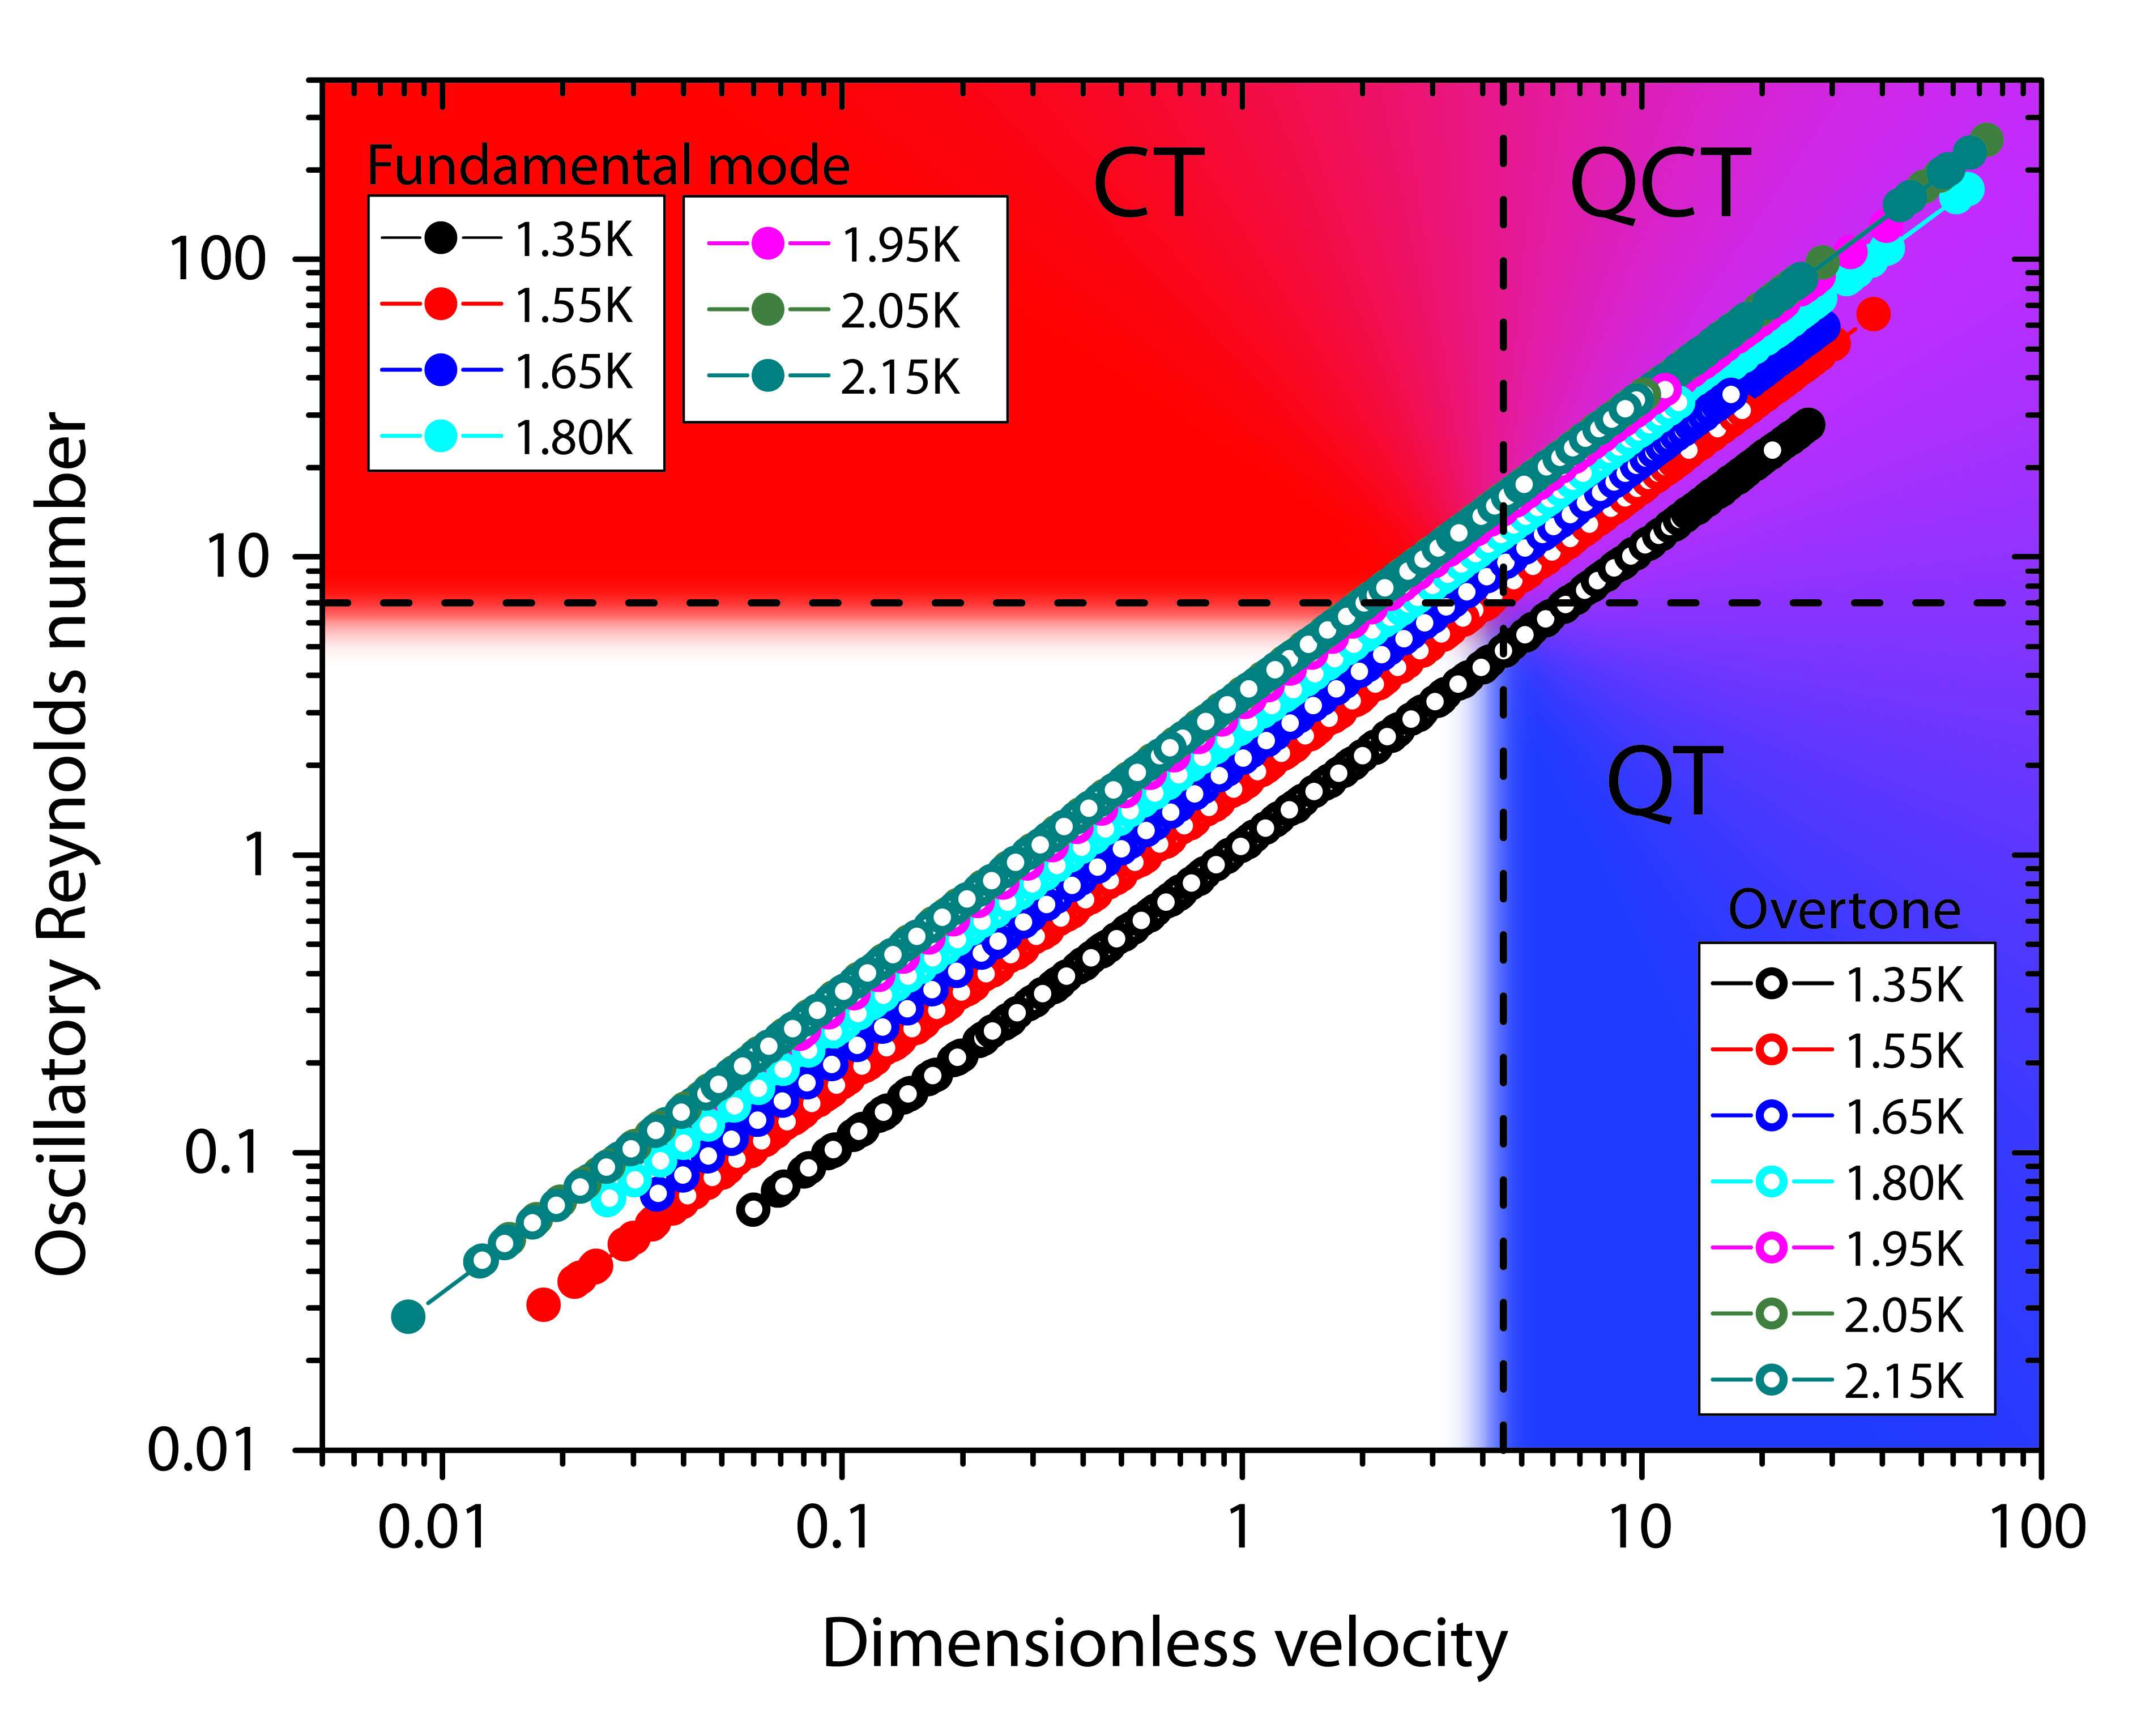
\includegraphics[width=1\textwidth]{graphs/FlowPhase_diagram}
	\caption{The simplified flow phase diagram illustrating the basic conditions for CT and QT to occur in the flow due to the investigated tuning fork. We note that only in the case of $ 1.35\unit{K} $ curve we are absolutely sure that QT arose as the first. The vertical and horizontal \textit{black dashed lines} marks the level of critical oscillatory Reynolds number $ \text{Re}_{\delta_{\ind n}c}\approx 7$ and dimensionless critical velocity $ v_{\ind c}^{\ind f}/\sqrt{2\pi \kappa f_0^{\ind f}} \approx v_{\ind c}^{\ind o}/\sqrt{2\pi \kappa f_0^{\ind o}} \approx 4.5$. }
\end{figure}

In reality, not only the transition itself to CT or/and QT (and possibly help trigger) will affect on another, but one might also suspect that even the intensity of either type of turbulence will bear significant consequences for the other one, due to coupling of the two fluids via the mutual friction force. A more thorough analysis of these effects is clearly required and this topic will be subject of further experimental investigations in an improved realization of the experimental setup.
